% -*- coding: utf-8; -*-
% vim: set fileencoding=utf-8 :

% The paper on using Luau telemetry to measure the effectiveness of type error reporting.

\documentclass[english,submission,cleveref]{programming}
%% use 'submission' for initial submission, remove it for camera-ready (see 5.1)

\usepackage{todonotes}

%%\overfullrule=1mm

%% BEGIN tobias pape 2021-11-06
% Why do we need this? To have headings in the abstract.
\makeatletter
\newcommand*\abstractpart[1]{\unskip\par\noindent{\firamedium\color{P@GrayFG}{#1}}\enspace}
\makeatother
%% END

\usepackage{alltt}
% Not sure why <Programming> is recommending non-standard tools
% \usepackage[backend=biber]{biblatex}
\usepackage[export]{adjustbox}
\usepackage{amssymb}
\usepackage{calc}
\usepackage{colortbl}
\usepackage{listings}
\usepackage{mathpartir}
\usepackage{pifont}
% Errors with
% ! Undefined control sequence.
% <argument> \l__siunitx_number_implicit_plus_bool 
% l.61 \begin{document}
% using Mac TeXlive 20230313_2
% \usepackage{siunitx}
\usepackage{tikz}
\usepackage{subcaption}
\usepackage{wasysym}
\usepackage{xcolor}
\usetikzlibrary{shapes.geometric}

%%%%%%%%%%%%%%%%%%
\paperdetails{
  %% perspective options are: art, sciencetheoretical, scienceempirical, engineering.
  %% Choose exactly the one that best describes this work. (see 2.1)
  perspective=scienceempirical,
  %% State one or more areas, separated by a comma. (see 2.2)
  %% Please see list of areas in http://programming-journal.org/cfp/
  %% The list is open-ended, so use other areas if yours is/are not listed.
  area={Data mining for programming, Telemetry},
  %% You may choose the license for your paper (see 3.)
  %% License options include: cc-by (default), cc-by-nc
  % license=cc-by,
}
%%%%%%%%%%%%%%%%%%

%%%%%%%%%%%%%%%%%%
%% These data are provided by the editors. May be left out on submission.
%\paperdetails{
%  submitted=2023-1-31,
%  published=2016-10-11,
%  year=2016,
%  volume=1,
%  issue=1,
%  articlenumber=1,
%}
%%%%%%%%%%%%%%%%%%

\begin{document}

\title{Type Error Telemetry at Scale}
% lean, lite, modest, non-intrusive, private, ...
% {Millions of Type Errors} = 72M forced strict, 1/2M type error is disappointing!
%% \subtitle{Impersonal Telemetry to Measure User Experience}

%\titlerunning{DRAFT do not distribute}

% Alphabetical order for authors?

\author[a,b]{Ben Greenman}
\authorinfo{(\email{benjamin.l.greenman@gmail.com}) was a CIFellows 2020
postdoc at Brown Univesity and is now an assistant professor
at the recently-named Kahlert School of Computing at the University of Utah.}
\affiliation[a]{Brown University, Providence, RI, USA}
\affiliation[b]{University of Utah, Salt Lake City, UT, USA}
% \orcid{0000-0001-7078-9287}

\author[c]{Alan Jeffrey}
\authorinfo{(\email{ajeffrey@roblox.com}) is a Principal Software Engineer at Roblox.}
% \orcid{0000-0001-6342-0318}
\affiliation[c]{Roblox, San Mateo, CA, USA}

\author[a]{Shriram Krishnamurthi}
% \orcid{0000-0001-5184-1975}
\authorinfo{(\email{shriram@brown.edu}) is the Vice President of Programming Languages (no, not really) at Brown University.}

\author[c]{Mitesh Shah}
\authorinfo{(\email{mshah@roblox.com}) is Senior Engineering Director, Programmability, at Roblox.}

%\renewcommand{\shortauthors}{...}

%\authorrunning{DRAFT do not distribute}

\newcommand{\code}[1]{\texttt{#1}}
\newcommand{\FILL}{\textbf{FILL}}
\newcommand{\dotscale}[1]{\scalebox{0.72}{#1}}
\newcommand{\wideas}[2]{\makebox[\widthof{#2}][l]{#1}}
\newcommand{\twoline}[2]{\parbox[s]{1.4cm}{\flushleft#1\newline#2}}
\newcommand{\chkYes}{\dotscale{\CIRCLE}}
\newcommand{\chkMaybe}{\wideas{\dotscale{\Circle}}{\chkYes}}
\newcommand{\chkNo}{\wideas{}{\chkYes}}
\newcommand{\pct}[1]{\SI{#1}{\percent}}
\newcommand{\percentile}[1]{{#1}th~percentile}
\newcommand{\modefont}[1]{\texttt{#1}}
\newcommand{\mnocheck}{\modefont{nocheck}}
\newcommand{\mnonstrict}{\modefont{nonstrict}}
\newcommand{\mstrict}{\modefont{strict}}
\newcommand{\FS}{background}
\newcommand{\zerowidth}[1]{\makebox[0pt][l]{#1}}
\newcommand{\nK}[1]{#1\textsc{k}}
\newcommand{\stddev}[1]{[\nK{#1}]}
\newcommand{\gcell}[1]{\cellcolor{green!20}#1}
\newcommand{\ycell}[1]{\cellcolor{yellow!18}#1}
\newcommand{\ocell}[1]{\cellcolor{orange!29}#1}
\newcommand{\rcell}[1]{\cellcolor{red!30}$\!\!$#1$\!\!$}
\newcommand{\gbox}[1]{\colorbox{green!20}{#1}}
\newcommand{\ybox}[1]{\colorbox{yellow!18}{#1\vphantom{Ap}}}
\newcommand{\obox}[1]{\colorbox{orange!29}{#1\vphantom{Ap}}}
\newcommand{\rbox}[1]{\colorbox{red!30}{#1\vphantom{Ap}}}
\newcommand{\tefsfont}[1]{\textsc{#1}}
\newcommand{\tekey}{\tefsfont{te}}
\newcommand{\fskey}{\tefsfont{fs}}
\newcommand{\QALAN}{\FILL{} Alan:}
\newcommand{\panon}{pseudonymized}

%%
%% The code below is generated by the tool at http://dl.acm.org/ccs.cfm.
%% Please copy and paste the code instead of the example below.

\begin{CCSXML}
<ccs2012>
<concept>
<concept_id>10002944.10011123.10010916</concept_id>
<concept_desc>General and reference~Measurement</concept_desc>
<concept_significance>500</concept_significance>
</concept>
</ccs2012>
\end{CCSXML}

\ccsdesc[500]{General and reference~Measurement}

\keywords{types, gradual typing, telemetry, user study, large-scale study}

\maketitle

\begin{abstract}
  \let\paragraph\abstractpart

  \paragraph{Context}
  %% What is the broad context of the work? What is
  %% the importance of the general research area?
  {Roblox Studio} lets millions of creators
  build interactive experiences by programming in a variant
  of Lua called Luau.
  The creators form a broad group, ranging from novices writing
  their first script to professional developers; thus, Luau
  must support a wide audience.
  As part of its efforts to support all kinds programmers, Luau includes an
  optional, gradual type system and goes to great lengths to minimize false
  positive errors.

  \paragraph{Inquiry}
  %% What problem or question does the paper
  %% address? How has this problem or question been
  %% addressed by others (if at all)?
  Since Luau is currently being used by many creators, we want to collect their feedback
  to improve the language and, in particular, the type system.
  The standard way to collect feedback at a large scale from creators working on
  real projects is to deploy client-side telemetry; however, we cannot
  scrape personal data or proprietary information, which means we cannot
  collect source code fragments, error messages, or even filepaths.
  The research questions are thus about how to conduct telemetry that
  is not invasive and obtain insights from it about type errors.

  \paragraph{Approach}
  %% What was done that unveiled new knowledge?
  We designed and implemented a pseudonymized, randomized telemetry system for Luau.
  Telemetry records include a timestamp, a session id, a reason for sending,
  and a numeric summary of the most recent type analyses.
  This information lets us study type errors over time
  without revealing private data.
  We deployed the system in Roblox Studio during Spring 2023
  and collected over 1.5 million telemetry records from over 340,000 sessions.

  \paragraph{Knowledge}
  %% What new facts were uncovered? If the
  %% research was not results oriented, what new
  %% capabilities are enabled by the work?
  We present several findings about Luau, all of which suggest that telemetry
  is an effective way to study type error pragmatics.
  One of the less-surprising findings is that opt-in gradual types are unpopular:
  there is an 100x gap between the number of untyped Luau sessions and the number
  of typed ones.
  One surprise is that the strict mode for type analysis is overly conservative
  about interactions with data assets.
  % Instead of using the flexible dynamic type, it uses a top type and requires
  % creators to down-cast assets.
  A reassuring finding is that type analysis rarely hits its internal limits on
  problem size.

  \paragraph{Grounding}
  %% What argument, feasibility proof, artifacts,
  %% or results and evaluation support this work?
  Our findings are supported by a dataset
  of over 1.5 million telemetry records.
  The data and scripts for analyzing it will be available in an artifact.

  \paragraph{Importance}
  %% Why does this work matter?
  Beyond the immediate benefits to Luau,
  our findings about types and type errors have implications
  for adoption and ergonomics in other gradual languages
  such as TypeScript, Elixir, and Typed Racket.
  Our telemetry design is of broad interest, as it reports on
  type errors without revealing sensitive information.

\end{abstract}


\section{Introduction}
\label{s:introduction}

{Roblox} is a platform for {shared virtual experiences} (typically 3D games), with
65~million Daily Active Users, and 14~billion hours of engagement in
April--June 2023~\cite{corp.roblox.com}.
There are over 5~million distinct user-created programs available on the platform thanks to a
worldwide community of 3~million creators.
Many of the creators program for fun or learning and may
not consider themselves software developers; others are professional
developers.

Creators program using the
{Luau} programming language~\cite{luau-lang.org},
an extension of {Lua~5.1~\cite{lua}}.
The main addition in Luau is a static type system that infers
types for all Luau programs on the fly, as creators modify the code.
These types are used primarily in IDE tooling such as autocomplete and
in API documentation~\cite{luau-autocomplete}, and indeed, creators
may be unaware that a typechecker is analyzing their code.
However, creators can opt in to receiving type error reports and they can write
their own types to guide designs and document their intentions.

Due to the broad community of creators, the goals of the Luau type
system are rather unique~\cite{bfj-hatra-2021}.
Whereas a traditional type system focuses on compilation and memory
safety, Luau takes a lenient approach by default and lets creators
gradually~\cite{st-sfp-2006,tf-popl-2008} migrate to rigorous checks
one module at a time.
In this way, for example,
students in code camps may begin in the \mnocheck{} mode that reports only
syntax errors; hobbyists can use \mnonstrict{} mode to identify
would-be runtime errors; and developers who need to ensure software
quality can rely on \mstrict{} mode.
(No matter the mode, a {\FS{}} type analysis still drives the IDE tools.)
Luau's types aim to support untyped designs, in the spirit of migratory
typing~\cite{tfffgksst-snapl-2017}, so that creators can switch modes without
needing to restructure their code in major, potentially-breaking, ways.

In this paper, we investigate methods for measuring the effectiveness
of the {Luau} type system.
The goal is to collect feedback at a large scale, with thousands
of participants maintaining real codebases.
Consequently, the measurements cannot reveal \emph{any} information about
source code, as it may contain personal data, proprietary algorithms, novel
game designs, and so on.
In comparison to prior work~(\cref{s:related}), which
with few exceptions~(e.g.,\cite{hlzbr-ecoop-2021}) is small in scale
or collects source code, we performed a large-scale study using \panon{}
{telemetry}.

Our starting point is a telemetry framework that is built in
to {Roblox Studio} and currently measures the effectiveness of
creation features.
This system randomly determines which sessions should report telemetry, and,
for those sessions, reports telemetry records back with a summary of the
session.

In this work, we design telemetry that collects data on type errors without
exposing source code, source locations, or even error message text (which
may contain revealing information).
The telemetry counts the number and \emph{kind} of type errors at various
levels of granularity.
Furthermore it maintains a client-side approximation of the latest source-code
edits and uses that to identify type errors that overlap with this edit range.
Telemetry records are correlated by session, using a \panon{} session
identifier and a timestamp.

With this telemetry data, we investigate research questions about
the adoption and benefits of type analysis:
\begin{description}
  \item[RQ1.]
    How many creators use type analysis?
    How often do projects contain modules with different
    analysis modes?
    How often do creators turn analysis off?
  \item[RQ2.]
    For modules that use type analysis:
    which errors arise,
    how do creators respond,
    and which errors tend to persist despite subsequent edits?
  \item[RQ3.]
    What impact does type analysis have on the number of \FS{}
    errors?
    For example, do \FS{} errors pile up in unanalyzed projects?
\end{description}

Beyond their immediate revelance to {Luau},
answers to these questions have broad implications for the design
of gradually-typed languages.
Luau represents a large-scale combination of ideas from
gradual typing~\cite{st-sfp-2006,tfffgksst-snapl-2017,bat-ecoop-2014},
success typing~\cite{lindahl2006practical},
and semantic subtyping~\cite{CF05:GentleIntroduction,Jef22:SemanticSubtyping}.
Lessons from this experience can inform future applications.

At a higher level, this paper is the first to use telemetry 
to study a type checker.
It thus represents a step toward data-driven language design,
informed by many users' actual practice.
Our data captures over 340,000 sessions
that occured between February and April 2023
and covers thousands of type analysis errors
and millions of \FS{} errors.
By contrast to typical qualitative methods such as surveys and interviews, it
is not restricted to users' \emph{perceptions} about their work and it is not
limited to a small number of users.


\paragraph{Contributions}
\begin{itemize}
  \item
    Design of a low-overhead telemetry system
    that reports on type errors without revealing source code.

  \item
    Lessons from many thousands of type errors about
    adoption, persistent errors, and creators' responses.

  \item
    An available dataset of over 1.5 million telemetry records
    and scripts to analyze them.
    \emph{We intend to submit this in an artifact.}

\end{itemize}


\section{Context: {Roblox} and {Luau}}
\label{s:context}
% https://create.roblox.com/docs/scripting/luau

% TODO quick reference table
% \begin{table}
%   \caption{Modes and analyses}
%   \label{t:mode-analyze}
% 
%   Mode: nocheck ...
%   Analysis: nocheck ... forced strict
% 
% \end{table}

%% Most users of {Roblox Studio} do not opt in to type error
%% reporting (\pct{90},~\cref{s:data}), and so they do not see the ``squiggly underlining'' that
%% indicates a type error site. Nonetheless, the type inference system
%% still runs in the background (since it drives autocomplete and other
%% type-based tools), letting us see which type errors would have
%% been reported and whether users fix these errors over time.

{Roblox Studio} is a workbench that
combines {3D creation} tools and an Integrated
Developer Environment (IDE), as seen in \cref{fig:roblox-studio}.
The IDE includes an optional \emph{Script Analysis} widget that
reports syntax errors, type errors, and problems identified by
lint tools. The main editor widget can also highlight
source locations in code where reported errors occur.


\paragraph{Type Analysis Modes, \FS{} Analysis}

Creators can opt in to detailed error reports and highlights by
choosing a \emph{type analysis mode} for each script they write:
\begin{itemize}
  \item \mnocheck{}: report only syntax errors (the default),
  \item \mnonstrict{}: report syntax errors and a subset of high confidence type errors, or
  \item \mstrict{}: report syntax errors and all type errors.
\end{itemize}
Each run of type analysis can report several errors.
There is no guarantee that creators read every error.
In fact, creators who close the Script Analysis widget
will see highlights in their code but no further details.

In addition to the main type analysis, Roblox Studio takes a second pass over
every codebase with a \emph{\FS{}} analysis to infer autocomplete suggestions
and drive other IDE tools.
To infer precise types,
the \FS{} analysis uses rigorous checks very similar to those of
\mstrict{} mode (but not identical: see \cref{s:strict-vs-forcedstrict})
no matter what mode the creator declared for the script.
(Internally to Roblox Studio, this analysis is called \emph{forced strict}
because it ignores the creator's choice and applies strong checks.)
When it fails to infer a type, \FS{} analysis defaults to the unknown gradual
type~\cite{st-sfp-2006}.
Creators cannot see the errors reported by \FS{} analysis.

As an example of \mnonstrict{} mode, the following program only reports one error:
\begin{verbatim}
  --!nonstrict
  local x = { p = 5, q = nil }
  if condition then x.q = 7 end
  local y = x.p + x.q --> OK
  local z = x.r           --> UnknownProperty: Key 'r' not found in table 'x'
\end{verbatim}
In \mstrict{} mode, it reports two errors:
\begin{verbatim}
  --!strict
  local x = { p = 5, q = nil }
  if condition then x.q = 7 end
  local y = x.p + x.q --> TypeMismatch: Type 'nil' could not be converted into 'number'
  local z = x.r           --> UnknownProperty: Key 'r' not found in table 'x'
\end{verbatim}
In cases like this, where it is undecidable whether there will be a run-time error,
\mstrict{} mode errs on the side of reporting an error, and \mnonstrict{} mode errs on
the side of suppressing the error.

Both modes report the \code{UnknownProperty} error because
misspellings of property names are common enough to report in both
\mstrict{} and \mnonstrict{} mode. See~\cite{bfj-hatra-2021}
for a more detailed discussion of the rationale for \mstrict{} and
\mnonstrict{} mode.

\begin{figure}[t]\centering
  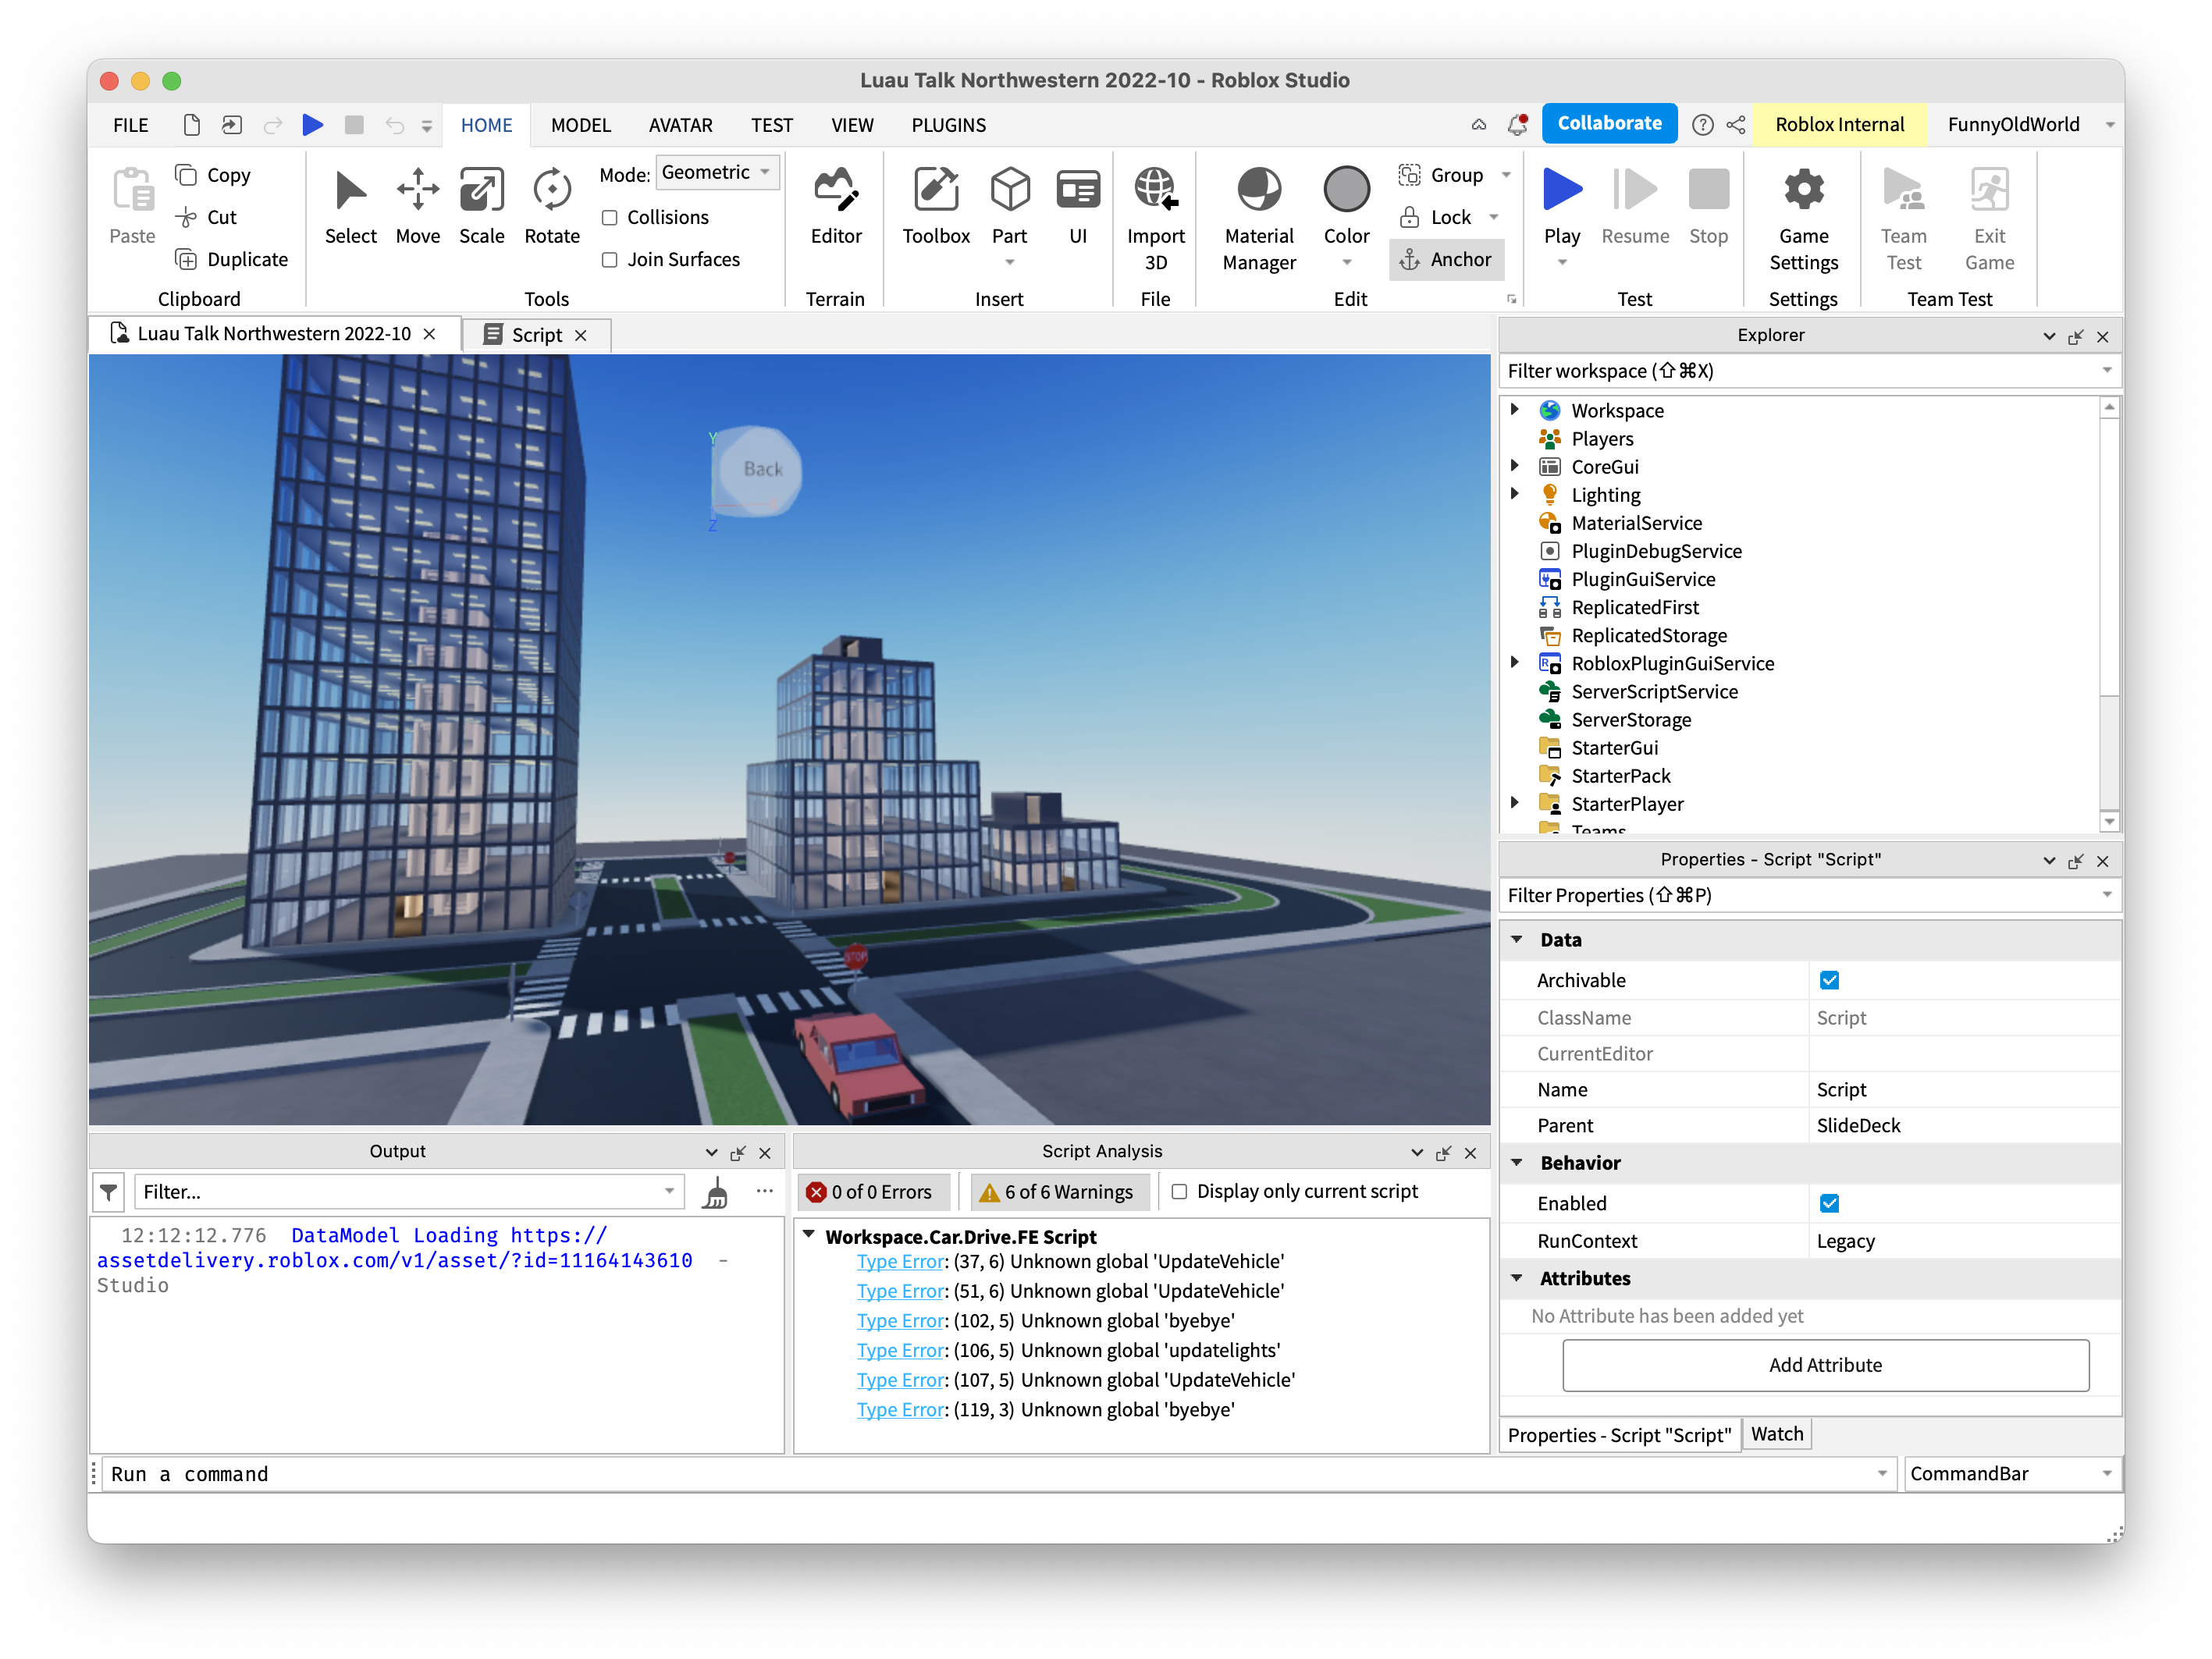
\includegraphics[width=.45\textwidth]{img/roblox-studio.png}
  \includegraphics[width=.45\textwidth]{img/roblox-studio-ide.png}
  \caption{{Roblox Studio 3D creation} tools (left) and IDE (right).}
  \label{fig:roblox-studio}
\end{figure}

\Cref{t:type-error-labels} lists a few of the type errors that
script analysis can report (10 out of 35 total)
to give a sense of Luau.
A \code{SyntaxError} is the only error that can appear in
\mnocheck{} code.
Several errors in addition to \code{UnknownProperty} are about
tables, which are Luau's (and Lua's) primary data structure.
Tables support arrays, dictionaries, and objects; consequently,
tables can have methods and can usually be extended.
The error \code{TypesAreUnrelated} is a special kind of type mismatch
that arises only during cast, unification, or subtyping check.
A \code{CountMismatch} occurs when the arguments to a function
do not match the function's arity.
Similarly, an \code{IncorrectGenericParamCount} is an arity mismatch
for a generic type.
Lastly, \code{CodeTooComplex} occurs when the typechecker hits an
internal limit on problem size and \code{GenericError} is a catch-all
label for miscellaneous errors.
When Luau can provide more context regarding a generic error, it uses
a second error label called \code{ExtraInformation} to attach
a brief description.

\begin{table}
  \caption{Sample type errors.}
  % https://github.com/Roblox/luau/blob/master/Analysis/include/Luau/Error.h
  %% from type analysis, but they're not all really type errors
  \label{t:type-error-labels}

  \begin{tabular}{ll}
    Label & Interpretation \\\midrule
    \code{TypeMismatch} & Basic type error. \\
    \code{SyntaxError} & Basic parse error, e.g., \code{for if end}. \\
    \code{UnknownProperty} & Referenced an invalid field or method.  \\
    \code{OnlyTablesCanHaveMethods} & Tried to attach a method to a non-table. \\
    \code{CannotExtendTable} & Tried to extend a sealed table. \\
    \code{TypesAreUnrelated} & Failed cast, unify, or subtype. \\
    \code{CountMismatch} & Arity mismatch for a function. \\
    %% \code{CannotCallNonFunction} & Called a value that is not a function. \\
    \code{IncorrectGenericParamCount} & Arity mismatch for a generic type. \\
    \code{CodeTooComplex} & Type analysis failed, cannot understand the code. \\
    %% \code{UnificationTooComplex} & Type analysis failed, unification solver hit a limit \\
    \code{GenericError}
    & Generic label for other non-type errors, such as\\
    & \hbox{}~~looping over an unordered table.
    %% attempting to extend a type that does not describe a class
    %% attempting to iterate over a table without a clear order

  \end{tabular}
\end{table}

\paragraph{On-the-Fly Typechecking}

Scripts come in two flavors: \emph{module scripts} and \emph{non-module
scripts}.
Module scripts provide reusable libraries, which may be
{imported} by other scripts.
Module scripts therefore form a graph in general,
though it is an error in \mstrict{} mode to create an import cycle
and edges are removed to make the graph acyclic.
%% \QALAN{}: do all modes remove the edges?

Typechecking analyzes the entire module graph, but it also keeps track of which
modules have been edited to avoid repeating work.
Any script that the creator modifies gets marked as dirty,
and any script that is dirty or that transitively imports a dirty
module gets analyzed by the typechecker.
In the common case when typechecking is performed for autocomplete,
only the current script gets checked because it is the only dirty
script, and because nothing it requires can transitively require it, since
the module graph is acyclic.
With this strategy, the typechecker can run after every keystroke without
slowing down Roblox Studio.


\paragraph{Data Model}

The state of the world in a {Roblox} program is captured by
the \emph{data model}, which is a tree of {instances}, such as
parts, models, meshes, effects, lighting, audio assets, and physics
constraints such as forces, springs and joints.
Each asset lives in a separate file.
There may be thousands of assets.
%% The data model can be seen in the Explorer view of~\cref{fig:roblox-studio}.
%% \QALAN{} where is it? very hard to see, needs a clear label

While a program is under development, it is typical for the data
model to be edited.
% For example, instances may be added or renamed.
% --> Commented out to get a better page break.
Since the shape of the data model tree is reflected in
the type system, it is possible for these edits to introduce a mountain
of type errors across the project.


\section{Telemetry Design}

\subsection{Limits of Telemetry}

Telemetry allows an application to ``phone home'' with data
summarizing usage patterns, such performance data, crash reporting,
and feature uptake. A typical usage is in deciding whether an API can
be deprecated: without telemetry it may be difficult to know how
popular it is, but with telemetry it is
straightforward.

IDEs use telemetry in a similar fashion\todo{I really don't know what
  this means. Are you saying VSCode is constantly calling home? Is it
  telling Racket about my API usage? Do we need anything in this para?} to most user-facing
applications, for example VSCode~\cite{vsc-telemetry} and
IntelliJ~\cite{intellij-telemetry} report telemetry.
See~\cref{s:related} for futher comparisons among telemetry designs.

Telemetry for programming languages can be controversial:e.g., see
the lively discussion around telemetry in the Go
toolchain~\cite{golang-telemetry}. 
The Luau open source toolchain does \emph{not} report telemetry,
as it is designed to be used in build environments such as Continuous Integration
servers, where hermetic deterministic builds are expected.

Telemetry therefore faces at least two major constraints:
\begin{itemize}

\item It should not reveal private information. This can include
  Personally Identifying
  Information (PII) about creators: their identity, location, etc. It also
  includes trade secrets. Even an error message that contains the name
  of a function could reveal something the creator would not want to
  share.

\item For performance reasons, it should have minimal run-time
  overhead and also transmit small and bounded amounts of data.
\end{itemize}
Cox discusses in detail the privacy implications and tradeoffs
in telemetry~\cite{transparent-telemetry}.

% BEN: I believe the above subsumes all of the below:
% Much of the concern about telemetry is because of its potential impact on
% privacy. It can not only reveal Personally Identifiable Information
% (PII) but also trade secrets, etc. Thus, telemetry should not reveal
% PII, source code, error messages (which can refer to source), the
% creator's identity, and so on.
% % and no information about what creation the data came from.

% For performance reasons, there are limits to telemetry data:
% telemetry records have size limits, and the performance impact of
% recording telemetry should be minimal.

% In summary, the limitations of telemetry are:
% \begin{itemize}
%   \item Data that don't reveal private information.
%   \item Fixed-size telemetry records.
%   \item Minimal overhead to record telemtry.
% \end{itemize}

In addition, due to the architecture of Roblox Studio
there is some information that is not available to the
typechecker:
\begin{itemize}
  \item The typechecker does not have access to some lifecycle events,
    such as save, quit and publish.
  \item The typechecker does not have access to GUI state, for example
    whether the Script Analysis widget is visible.
\end{itemize}

\subsection{Telemetry Records}
\label{s:telemetry-records}

\begin{figure}[t]\centering
  % BEN: The left brace is confusing. Is ID not fixed?
  \begin{tabular}{|l|l|l|l|l|l|l|}\hline
    ID & Time & Mode & Reason & Size Info & Overall Counts & Edit Range Counts
    \\\toprule
    \multicolumn{6}{c}{\upbracefill} & \multicolumn{1}{c}{\upbracefill} \\[-0.5ex]
    \multicolumn{6}{c}{fixed-size} & \multicolumn{1}{c}{variable-size}
  \end{tabular}
  \caption{Structure of a telemetry record. There are 13 overall counts and up to 70 edit range counts in each record.}
  \label{f:tdata}
\end{figure}

The telemetry for a Roblox Studio session is gathered as a series of
records, all with the same \panon{} session
identifier. This allows us to correlate telemetry across a single
session, but not between sessions.

In order to avoid swamping our telemetry servers, we randomly throttled
the generation of telemetry records:
\begin{itemize}
  \item
    1\% of Roblox Studio sessions were enrolled in generating telemetry, and
  \item
    0.5\% of runs of the typechecker (approximately 1 in 200 keystrokes)
      in an enrolled session generated a telemetry record.
\end{itemize}
In order to find how file-switching correlated with type errors, we
additionally recorded
every run of the typechecker in an enrolled session which switched
file generated a telemetry record.\todo{I cannot parse this!}

\Cref{f:tdata} shows the structure of our telemetry records:
\begin{enumerate}
  \item
    ID: a \panon{} identifier for the current session.
  \item
    Time: one timestamp from the client and one from the server.
    %% timestamp explanation \cref{s:data-cleaning}
  \item
    Mode: type analysis mode of the current file: \mnocheck{},
    \mnonstrict{}, or \mstrict{}.
  \item
    Reason: a flag that explains whether this record was sent due to a
    randomly-selected keystroke or a module switch.
  \item
    Size Info: number of lines in the codebase and number of lines in the edit range.
  \item
    Overall Counts: summarizes type errors and \FS{} errors during the
    last two invocations of type analysis, and additionally reports the number
    of times type analysis hit an internal limit on problem
    size~(see~\cref{s:code-too-complex} for details).
    For each invocation and each kind of
    analysis error, there are three summary counts:
    %% grand total = 12
    \begin{itemize}
      \item total number of errors,
      \item errors in the current module, and
      \item errors in the current edit range.
    \end{itemize}
  \item
    Edit Range Counts: these list specific errors that arose in the last two
    type analyses and overlap with the current edit range.
    Since there are 35 possible errors~(\cref{s:context}), there can be up to 70 counts
    in a telemetry record.
    Exactly how to interpret this data depends on which analysis it came from:
    \begin{itemize}
      \item
        Errors in the latest type analysis are currently visible to the
        creator.
        These may have been introduced by the changes in the edit range.
      \item
        Errors from the previous type analysis were visible before the creator
        made the latest edits.
        These may have motivated some of the changes in the edit range.
    \end{itemize}
\end{enumerate}




To track the edit range, we record a start and end position, which we
update appropriately on every edit. This can result in very large edit
ranges, for example, if the user edits at the beginning and end of the
file.
The main benefit of this strategy is that it ensures constant-size telemetry records.

\paragraph{NOTES} %% FILL
This kind of telemetry data is coarse-grained.
For instance, it does not let us distinguish between edits that ignore a type
error from edits that remove one error while introducing another.
We acknowledge this and other threats in~\cref{s:threats}.
The main advantages of the telemetry design are the small size of each record
and complete the lack of PII.
Furthermore, despite the limitations, Studio's telemetry supports a variety of
interesting conclusions that we showcase in the next section.


\section{The Data}
\label{s:data}

Roblox Studio collected type error telemetry in Spring 2023,
between February and April.
Every Studio session had a small random chance of generating
telemetry~(\cref{s:telemetry-records}).
The chosen sessions generated a record whenever the user switched modules and
randomly on each keystroke.
In total, we collected 1.5 million telemetry records.
Roughly two-thirds of records are due to keystrokes.

\Cref{f:records-per-hour} provides a time-ordered distribution of the data.
Each vertical bar counts the number of records generated per hour according to
a client-side timestamp.\todo{Do we need all this detail?}
The bars are labeled with a California time zone because that is the locale of
the Roblox servers, which parsed the timestamps.
Most buckets contain roughly one thousand records, but some have very few
and a handful of others exceed three thousand.
%% \FILL{} investigate one tower, what's happening?? all one session?
There is a sharp drop in early April when the experiment was finished
and the telemetry probe was removed (though there is a long tail as
developers uopdated Roblox Studio).
We do not know which timezone the records originated in, but since the counts
tend to peak midday California time it seems that the majority
of Roblox developers are following a Western Hemisphere schedule.
The counts for weekends (shaded regions) are often the tallest,
as Roblox has a significant school-aged creator community.

\begin{figure}[t]\centering
  %% TODO bigger text
  %% TODO weird artifact (|) in x-min label
  %% code/row-distribution.rkt
  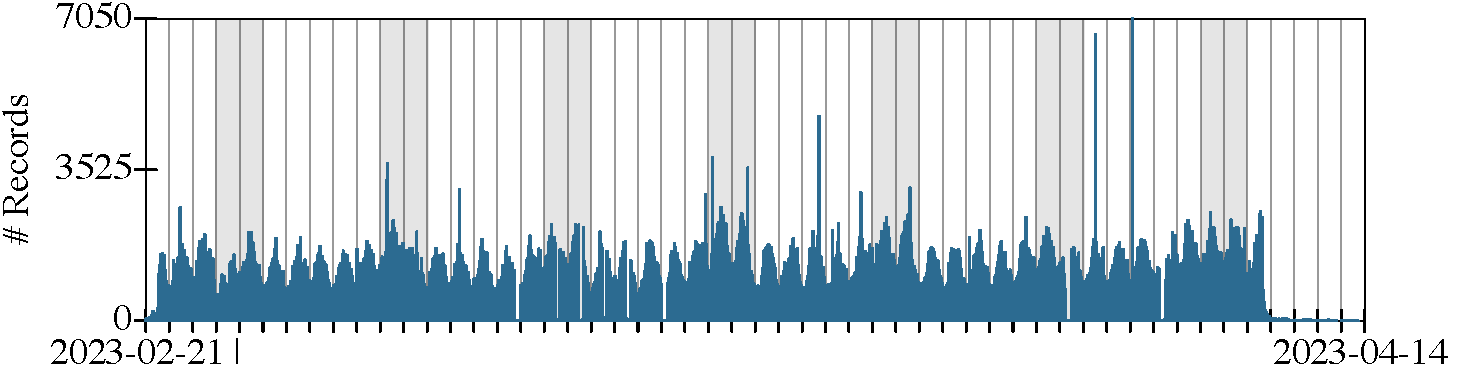
\includegraphics[width=\columnwidth]{img/row-distribution.pdf}
  \begin{tabular}{ll}
    Reason for sending:
    &
    \begin{tabular}[t]{r@{~~}l@{~~}r}
      996,164 & due to keystrokes  & [\pct{66.20}] \\
      508,572 & due to module switch & [\pct{33.80}]
    \end{tabular}
  \end{tabular}
  \caption{Telemetry records per hour. Each tick on the $x$-axis marks the start of a new day in California. Shaded ranges correspond to weekends.}
  \label{f:records-per-hour}
\end{figure}


\subsection{Data Cleaning}
\label{s:data-cleaning}

A close inspection of the data revealed a few anomalies.
For the most part, we omit the strange data from futher
analysis.\todo{I'm inclined to rewrite this to be much more concise.}\todo{agreed}

First, some records have odd timestamps according to the server's records.
Every telemetry record comes with two timestamps: a client-side timestamp
from when Roblox Studio created it and a server-side timestamp from when
the server posted it to its database.
The server timestamps are little use for our analysis because they bunch
together; it is common for several records to have identical server
timestamps.
However, server timestamps are useful for auditing because they should
be relatively close in value to the client timestamps.
For a small number of records (<100? \FILL{}), though, the client is off by a large
margin: up to one week behind and up to one day ahead of the server.
We attribute the large delays to issues when sending telemetry (lost internet
connection, etc.) and smaller offsets to incorrect time settings on the client
machine.
In any event, we do not filter these records from further
analysis.\todo{To be clear, you do NOT filter? Because the section is
  about what you DO filter.}

Second, some records have identical (client) timestamps.
This can happen legitimately if type analysis runs several times
in the same millisecond, but it is unlikely that a human would
enter keystrokes or switch modules quickly enough.
We keep the first record with a distinct timestamp and discard the others.
%% TODO wait, better deduplicate by session and not globally!!!

%% out/negative-edit-range.txt
%% actual value is NOT negative, but large positive over 4 billion
%% example: 4294967293
Third, the edit ranges are negative in a few hundred records~(1,533).
This is likely due to the user deleting a large block of code.
Since the issue affects so few records, we omit the negative ranges
from analysis (but, we do use other parts of the records; for example
the timestamps influence~\cref{f:records-per-hour}).

\subsection{Overall Size and Shape}

Three important characteristics of the recorded data are the size of the codebases,
the length of the sessions, and the number of type
errors.
We discuss these in turn.
Codebase size and session length follow power-law
distributions,\todo{Please confirm w/ a statistical test. See Clauset
  et al.: arXiv:0706.1062.} with
many small items and a few very large items.
The number of type analysis errors is somewhat low~(explained in the next
section), but sufficient to proceed with futher analysis.


\paragraph{Codebase Size}
%\label{s:codebase-size}

\begin{figure}[t]\centering
  % ;; (list* (max* vv) (median < vv) mm (stddev/mean mm vv) (percentile* vv)))
  % ;; percentile* = 0.95 -- 0.99
  % #hash((editrange . (1156036 926 3007043/817 30975.40553032358 (0.95 8220) (0.96 9858) (0.97 13656) (0.98 18956) (0.99 34725)))
  %       (event-count . (6079 138 38689/135 582.5752201972966 (0.95 960) (0.96 1174) (0.97 1304) (0.98 1836) (0.99 3302)))
  %       (files . (54884 7678 55257996/4639 11853.650098459446 (0.95 40029) (0.96 42771) (0.97 45417) (0.98 48688) (0.99 51761)))
  %       (lines . (1089963 3115 38928947/5992 22364.75846303099 (0.95 18561) (0.96 25892) (0.97 27014) (0.98 29725) (0.99 50547)))
  %       (timespan . (1387897376 845648 591343604248/185705 15724745.722577972 (0.95 10696064) (0.96 12715468) (0.97 15596940) (0.98 21153924) (0.99 35450460))))
  %% NOTE: 3 records have +1M lines, all from one nocheck session, all with 3 files
  %% - session "30,762,216,447,324"
  %% NOTE: 133 records have +52K files, all from one nocheck session
  %% - session "330,172,870,224,081" 
  %% (2nd biggest has 41K files "31,650,473,913,529")

%% Files has HUGE numbers thanks to data assets. Forget it.
% Files  &              &
% 11,911 & \stddev{12}  &
%  7,678 &              &
% 51,761 &              &
%   & 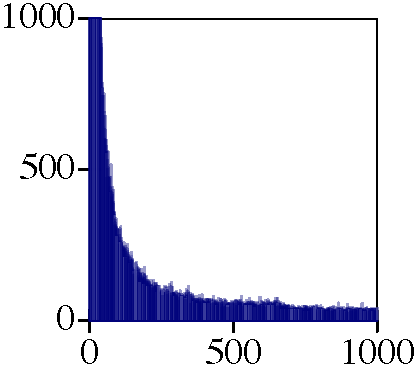
\includegraphics[width=0.2\columnwidth]{img/files-distribution.pdf}

%  \begin{tabular}{l@{}r@{~}l@{}r@{~}l}
%                 &  Lines &             &    Edit Range & \\
%    Mean [std]   &  6,497 & \stddev{22} &         3,680 & \stddev{31} \\
%    Median       &  3,115 &             &           926 & \\
%    \pct{99}     & 50,547 &             &        34,725 & \\
%    %% TODO x-axis starts at 1, not zero ... there are no zeros right??!
%      & 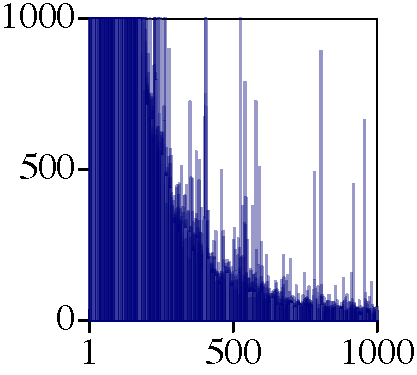
\includegraphics[width=0.2\columnwidth]{img/lines-distribution.pdf}
%    & & 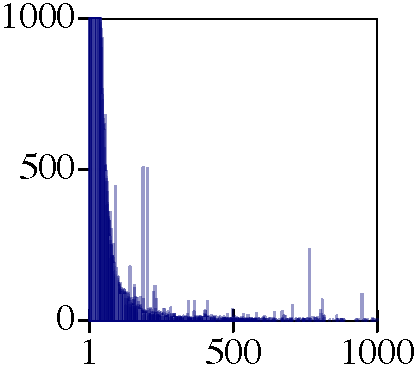
\includegraphics[width=0.2\columnwidth]{img/editrange-distribution.pdf}
%
%  \end{tabular}

  \begin{tabular}[t]{lrrrl}
    ~          & Mean [std] & Median & \pct{99} Pct. & Distribution \\
    Lines      & 6,497 \stddev{22} & 3,115 & 50,547 & 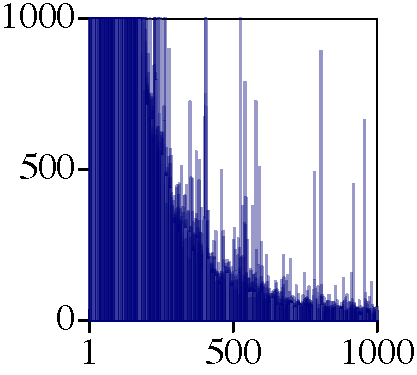
\includegraphics[width=0.14\columnwidth,valign=M]{img/lines-distribution.pdf} \\
    Edit Range & 3,680 \stddev{31} & 926   & 34,725 & 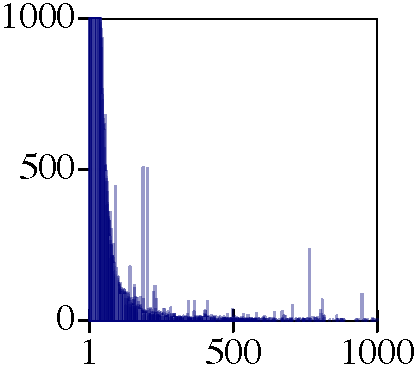
\includegraphics[width=0.14\columnwidth,valign=M]{img/editrange-distribution.pdf}
    %% TODO x-axis starts at 1, not zero
    %% TODO much bigger font or much smaller plot!!!

  \end{tabular}

  \caption{Size of analyzed code: number of files, number of lines, and lines in edit range}
  \label{f:codebase-size}
\end{figure}

\Cref{f:codebase-size} summarizes the size of projects in the dataset.
The top half of the figure reports the mean, standard deviation, median,
and \percentile{99} for the number of lines
and lines in edit range.\footnote{The data also contains the number of files in
each project, but these numbers are difficult to relate to typechecking because
projects may contain hundreds of files that define data assets.  For the
record, the median file count is 7,678 and the 99th percentile is 51,761 files.
}
The bottom half shows zoomed-in distributions of the line and edit range
sizes.
For example, the x-axis of the first plot ranges from 0 to 1,000 lines and
the y-axis counts up to 1,000 telemetry records.

There is a huge amount of variation across projects.
The largest ones have over 50,000 lines of code
while the smallest have merely 1 line of code.
Unsurprisingly, the numbers come with large standard
deviations~([std] in~\cref{f:codebase-size}).
The median values are more reasonable, with roughly 3,000 lines of code
and 1,000 lines in edit ranges.


\paragraph{Session Size}
%\label{s:session-size}

\begin{figure}[t]\centering
  %% NOTE max time = 1 million seconds = 15 days ...  +100 are over 2 days

%  \begin{tabular}{l@{}r@{~}l@{}r@{~}l} \\
%                 & Time Span (sec)  &       & Record Count  \\
%    Mean [std]   &     3,184 & \stddev{16}  &     286 & [583] \\
%    Median       &       845 &              &     138        \\
%    \pct{99}     &    35,450 &              &   3,302        \\
%    %% TODO x-axis starts at 1, not zero ... there are no zeros right??!
%    & 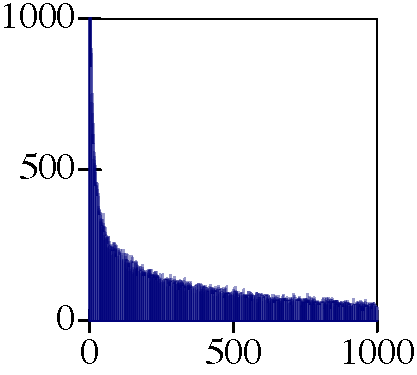
\includegraphics[width=0.2\columnwidth]{img/timespan-distribution.pdf}
%    & & 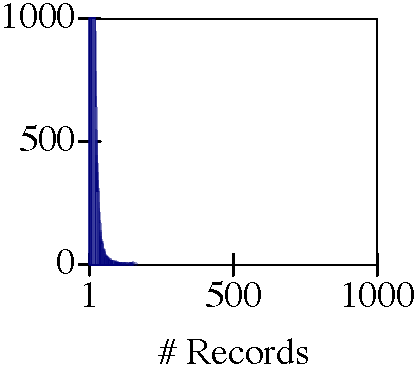
\includegraphics[width=0.2\columnwidth]{img/event-count-distribution.pdf}
%
%  \end{tabular}

  \begin{tabular}{lrrrl} \\
    ~               & Mean [std] & Median & \pct{99} Pct. & Distribution \\
    Time Span (sec) & 3,184 \stddev{16} & 845 & 35,450 & 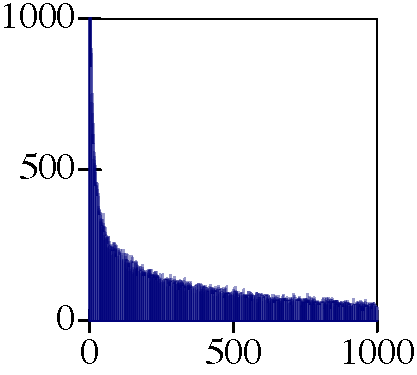
\includegraphics[width=0.14\columnwidth,valign=M]{img/timespan-distribution.pdf} \\
    Record Count    & 286 [583]         & 138 & 3,302  & 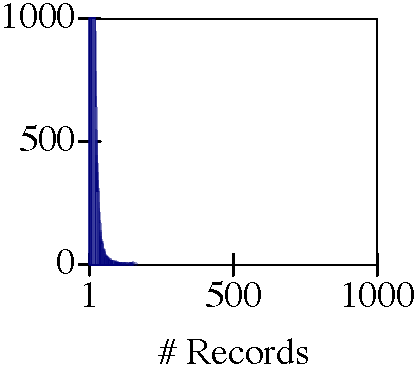
\includegraphics[width=0.14\columnwidth,valign=M]{img/event-count-distribution.pdf}
    %% TODO x-axis starts at 1
    %% TODO huge font, or smaller plot

  \end{tabular}

  \caption{Session size in seconds and in number of records.}
  \label{f:session-size}
\end{figure}

\Cref{f:session-size} outlines the size of the Roblox Studio sessions in the
data.
There are two useful notions of size: real time in seconds (between the first
and last record) and the total number of records.
The top of~\cref{f:session-size} reports the mean, standard deviation,
median, and \percentile{99}; the bottom shows size distributions, zoomed in
to focus on at most 1,000 units (x-axis) and 1,000 sessions
(y-axis).\todo{Again, confused.}

Similar to the data on project size, there is huge variation in session
length.
The longest sessions last several days and/or contain thousands of records,
while the shortest last a few milliseconds or include just one record.
Likewise, both plots in the figure follow a power-law distribution
(especially for record count).
A typical session runs on the order of minutes and consists of a few dozen events.
The median session time is approximately 14 minutes.
The median number of
records is 138.
% These numbers are reasonable.


\paragraph{Number of Type Analysis Errors}
%\label{s:count-analysis-errors}

\begin{figure}[t]
  \begin{tabular}[t]{ll} \\
    \begin{tabular}[t]{r@{~~}r@{~}l}
      595,137 & type errors \\
      289,698 & in current module & [\pct{48.68}] \\
       30,924 & in edit range & [\pct{5.20}]
    \end{tabular}
    \begin{tabular}[t]{r@{~~}r@{~}l}
      72,235,735 & {\FS{} errors} \\
      37,027,281 & in current module & [\pct{51.26}] \\
       1,111,178 & in edit range & [\pct{1.54}]
    \end{tabular}
  \end{tabular}
  \caption{Type errors and \FS{} errors across all telemetry records.}
  \label{f:count-analysis-errors}
\end{figure}

\FILL{} need old and current in edit range

\Cref{f:count-analysis-errors} lists the number of type analysis errors
and breaks them down by location in the codebase.
In total, there are over 590,000 type errors.
%% delete? upcoming figure has the same info
% Most of these (\pct{65}) appeared in modules that opted in to typechecking with either the
% \mnonstrict{} or \mstrict{} mode; the remainder are syntax errors reported
% by \mnocheck{} mode.
The number of \FS{} errors is much larger, 72M, because this analysis
ran on every module using strict type.
(Furthermore, \FS{} runs silently, so creators have no
awareness of or incentive to
fix these errors.)
Approximately half the analysis errors occurred in the current module,
and a small fraction overlapped with the current edit range~(\pct{5} for
type errors, \pct{1} for \FS{}).

The large fraction of errors in the current module is encouraging.
It suggests that errors appear locally, as the result of edits to nearby
code (as opposed to edits in one module raising errors in another), and
that creators fix the errors before switching focus to another
module.
The low fraction of errors in the edit range suggests that errors rarely
persist through nearby edits.


\subsection{Type Analysis Modes}
\label{s:type-analysis-modes}

\begin{figure}[t]\centering
  \begin{subfigure}[t]{\columnwidth}
    \begin{tabular}[t]{ll}
      %% FILL bar chart? rectangle?
      \begin{tabular}[t]{r@{~~}l@{~}r}
         1,341,348 & \mnocheck{}          & [\pct{89.14}] \\
           156,883 & \mnonstrict{}        & [\pct{10.43}] \\
             6,505 & \mstrict{}           & [\pct{ 0.43}]
      \end{tabular}
      \begin{tabular}[t]{r@{~~}l@{~~}r}
      \end{tabular}
    \end{tabular}
    \caption{Analysis modes across the 1,504,736 records.}
    \label{f:total-records}
  \end{subfigure}

  \begin{subfigure}[t]{\columnwidth}
    \begin{tabular}[t]{ll} \\
      \begin{tabular}[t]{r@{~~}r@{~}r}
        313,509 & \mnocheck{}   & [\pct{90.19}] \\
         32,902 & \mnonstrict{} & [\pct{ 9.47}] \\
            545 & \mstrict{}    & [\pct{ 0.16}] \\
            642 & mixed-mode    & [\pct{ 0.18}]
      \end{tabular}
      \begin{tabular}[t]{l@{~~}ll}
        %% TODO numbers may be off by +- 100
        %%    & 341 & contain a mode upgrade \\
        %%    & 320 & contain a mode downgrade \\
        %%    & 512 & contain modules with different modes
        %%  they don't match out/error-density*hasdown.rkt
        %%  ??? counting downs instead of sessions with downs ???
        %% TODO fix throughout paper!
        \zerowidth{Among the mixed-mode sessions:} \\
        & 176 & contain a mode upgrade \\
        & 233 & contain a mode downgrade \\
        & 512 & contain modules with different modes
      \end{tabular}
    \end{tabular}
    \caption{Analysis mode(s) for the 347,598 sessions.}
    \label{f:total-sessions}
  \end{subfigure}

  \caption{Overview of type analysis modes.}
  \label{f:dataset-overview}
\end{figure}

Creators have three analysis modes to choose from.
Furthermore, they can switch between modes at any time.
According to~\cref{s:type-analysis-modes}, however, usage is
extremely skewed toward the type-free \mnocheck{} mode.
Nearly \pct{90} of all records use the \mnocheck{} mode
and \pct{90} of all sessions use \mnocheck{} exclusively.
Among the rest, roughly \pct{10} of all records use \mnonstrict{} and only a
tiny fraction (\pct{0.4}) use \mstrict{}.
The per-session data is similar: \pct{9} use \mnonstrict{} exclusively
and \pct{0.2} use \mstrict{}.

These adoption numbers indicate that there is a communication gap;
as long as type checking is opt-in, most developers stay opted out.
Once Luau type checking is opt-out rather than opt-in, it will be interesting
to revisit these numbers.

%% mostly pure, rare mixes
Most sessions (\pct{99.82}) stick to a single analysis mode.
These sessions never change the mode in the current module and never switch
focus to a module with a different analysis mode.
Among the mixed-mode sessions, most (\pct{80}) switch to modules with
a different mode, about half contain at least one edit that upgrades
the typing strictness in the
current mode, and about half contain a downgrade.
There are 619 upgrades in total and 583 downgrades.
\FILL{} Ben check how often the downgrades follow the upgrades.


\paragraph{Are Upgrades Discouraging?}

%% 619 up-pairs, 583 down-pairs
%% === UP
%% min -3 max 57 median 0 mean 2.62 stddev 6.8390518952707335
%% === DOWN
%% min -48 max 30 median 0 mean -0.31 stddev 4.498748355271854

A possible explanation for the low adoption of \mnonstrict{} and
\mstrict{} mode is that upgrading to these modes leads to a large
number of type errors.
Creators might get discouraged or overwhelmed by a high error count and revert to
\mnocheck{} mode.

The data does not support this explanation.
On average, the mode-upgrades in the data resulted in 3 additional
type errors (stddev 7, median 0).
The worst-case increase was 57 type errors, which is very high
but exceptional.
In another exception, upgrading modes removed three type errors
(possibly due to other edits being rolled in with the
mode change).

In the other direction, mode downgrades have only a small negative effect on the
number of errors (mean -0.3, stddev 4, median 0, max -48).
%% curious outlier: downgrade added 30 errors!
We would see a much larger effect here if creators used downgrades
as a quick way to silence the typechecker.
But, creators evidently switch modes only when the code is already
in well-typed shape.


%% \paragraph{Module Switches vs Errors}
%% FILL need \%s out of all module switches.
%% How many module switches exit a module with errors?
%% > OLD DATA
%% > \mnocheck{} 24, \mnonstrict{} 9, \mstrict{} 3.
%% > Rare?
%% > More common for forcedstrict:
%% >  \mnocheck{} 190, \mnonstrict{} 16, \mstrict{} 2.
%% >
%% > How many module switches go to a module with errors?
%% > \mnocheck{} 70, nonstrict 9, strict 4
%% > For FS: \mnocheck{} 400, \mnonstrict{} 39, \mstrict{} 6.


\subsection{Errors by Mode}

\begin{figure}[t]\centering

  %%%% from nsa aggregate-tefs
  %% strict
  %%  te total 22771
  %%  mean 6.9 std 26.24592591869705 med 1 max 385
  %% 
  %%  fs total 114259
  %%  mean 34.9 std 155.41955823164017 med 1 max 4789
  %% 
  %% nonstrict
  %%  te total 362964
  %%  mean 2.3 std 66.44456626891912 med 0 max 13511
  %% 
  %%  fs total 7546175
  %%  mean 48.6 std 270.60578740369266 med 3 max 16712
  %%
  %% nocheck
  %%  te total 176309
  %%  mean 0.13 std 1.9040337635815197 med 0 max 289
  %% 
  %%  fs total 63784284
  %%  mean 47.7 std 885.8225471699477 med 1 max 251131

  \newcommand{\labelbars}[1]{\begin{tabular}[t]{l@{}l} \begin{tabular}[t]{r} \mnocheck{} \\ \mnonstrict{} \\ \mstrict{} \\ ~ \end{tabular} & #1 \end{tabular}}

    \begin{tabular}[t]{cc}
    %% TODO why text blurry??!
    Type errors & Background errors \\
    \labelbars{\includegraphics[valign=M]{img/error-by-mode-te.pdf}}
    & \labelbars{\includegraphics[valign=M]{img/error-by-mode-fs.pdf}}
  \end{tabular}
  \caption{FILL}
  \label{f:error-by-mode}
\end{figure}

\Cref{f:error-by-mode} shows how the type errors and \FS{} errors
in the data are split across type analysis modes.

Most type errors come from \mnonstrict{} mode, despite it having an order
of magnitude fewer users that \mnocheck{}.
This is unsurprising because \mnocheck{} reports only syntax errors,
whereas \mnonstrict{} reports several others kinds~(detailed in the next section).
Finally, \mstrict{} mode accounts for a small fraction of type errors, despite
being more picky, because so few creators use it.

Background analysis applies the same typechecker to every module, regardless
of mode, in the hope of enabling IDE tools.
Consequently, the breakdown of \FS{} errors matches the overall usage
data~(\cref{f:dataset-overview}): almost \pct{90} for \mnocheck{},
\pct{10} for \mnonstrict{}, and \pct{1} for \mstrict{}.
Type analysis finds a large number of errors in \mnocheck{} code;
unfortunately, we have no insight into whether those errors are true
positives or whether the analysis led to useful IDE suggestions.

\FILL{} average number of FS errors is
worst in \mnonstrict{}, 49, vs 48 nocheck and 7 strict.
median is 3 NS, 1 nocheck, 1 strict.
We might optimistically think that nocheck accumulates
lots of errors, but no that does not seem to be the case,
NS and nocheck both apparently fine with latent FS errors.


\subsection{Type Errors vs. Program Edits}
\label{s:type-error-survival}

\begin{table}[t]
  \caption{Number of telemetry records that add, keep, or drop (remove) specific type errors from their edit range.}
  \label{t:type-error-survival}
  \begin{tabular}{l@{}r@{}r@{}rr@{}r@{}rr@{}r@{}r}
    & \zerowidth{\mnocheck{}} & & & \zerowidth{\mnonstrict{}} & & & \zerowidth{\mstrict{}} & & \\
    & \rbox{Add} & \ybox{Keep} & \gbox{Drop} & \rbox{Add} & \ybox{Keep} & \gbox{Drop} & \rbox{Add} & \ybox{Keep} & \gbox{Drop} \\\midrule
    \code{CannotCallNonFunction} & {0} & {0} & {0} & {17} & {4} & {20} & {1} & {0} & {1} \\
    \code{CannotExtendTable} & {0} & {0} & {0} & {7} & {9} & {10} & {0} & {0} & {1} \\
    \code{CannotInferBinaryOperation} & {0} & {0} & {0} & {1} & {2} & {1} & {7} & {6} & {9} \\
    \code{CountMismatch} & {0} & {0} & {0} & {223} & {48} & {269} & {12} & {2} & {17} \\
    \code{DuplicateTypeDefinition} & {0} & {0} & {0} & {1} & {0} & {0} & {0} & {0} & {0} \\
    \code{FunctionDoesNotTakeSelf} & {0} & {0} & {0} & {4} & {6} & {5} & {0} & {0} & {0} \\
    \code{FunctionExitsWithoutReturn} & {0} & {0} & {0} & {9} & {3} & {6} & {11} & {5} & {8} \\
    \code{GenericError} & {0} & {0} & {0} & {206} & {52} & {203} & {8} & {1} & {9} \\
    \code{GenericExtraInformation} & {0} & {0} & {0} & {48} & {7} & {39} & {2} & {0} & {1} \\
    \code{IllegalRequire} & {0} & {0} & {0} & {16} & {3} & {33} & {0} & {0} & {2} \\
    \code{IncorrectGenericParamCount} & {0} & {0} & {0} & {0} & {0} & {0} & {1} & {0} & {1} \\
    \code{MissingProperties} & {0} & {0} & {0} & {11} & {3} & {11} & {6} & {4} & {6} \\
    \code{MissingUnionProperty} & {0} & {0} & {0} & {1} & {0} & {2} & {0} & {0} & {0} \\
    \code{ModuleHasCyclicDependency} & {0} & {0} & {0} & {20} & {9} & {15} & {0} & {0} & {1} \\
    \code{NotATable} & {0} & {0} & {0} & {7} & {2} & {8} & {2} & {0} & {1} \\
    \code{OccursCheckFailed} & {0} & {0} & {0} & {0} & {0} & {0} & {0} & {0} & {1} \\
    \code{OnlyTablesCanHaveMethods} & {0} & {0} & {0} & {1} & {0} & {2} & {0} & {0} & {0} \\
    \code{OptionalValueAccess} & {0} & {0} & {0} & {40} & {52} & {27} & {6} & {2} & {7} \\
    \code{SyntaxError} & {8349} & {314} & {19220} & {983} & {46} & {2658} & {16} & {0} & {71} \\
    \code{TypeMismatch} & {0} & {0} & {0} & {159} & {62} & {129} & {21} & {10} & {28} \\
    \code{TypesAreUnrelated} & {0} & {0} & {0} & {1} & {0} & {0} & {0} & {0} & {1} \\
    \code{UnknownPropButGotLikeProp} & {0} & {0} & {0} & {26} & {18} & {21} & {1} & {0} & {1} \\
    \code{UnknownProperty} & {0} & {0} & {0} & {347} & {180} & {385} & {19} & {19} & {35} \\
    \code{UnknownRequire} & {0} & {0} & {0} & {91} & {39} & {85} & {12} & {3} & {4} \\
    \code{UnknownSymbol} & {0} & {0} & {0} & {2348} & {496} & {2973} & {49} & {19} & {55}
  \end{tabular}

\end{table}

Equipped with an overall picture of the dataset and the skewed usage
of \mnocheck{}, \mnonstrict{}, and \mstrict{} modes, we are ready to explore
the type error data.
Our main focus is on the intersection between type errors
and edits to the programs.\todo{The next two sentences are in some
  sense our main RQs, right? I would call them out more explicitly and
  w/ more justification.}
When a type error highlights part of the code and the next edit range includes
that code, we want to know whether the error survives the edit.
Similarly, we want to know when an edit introduces a type error.

\Cref{t:type-error-survival} counts the number of times that types
errors overlap with the current edit range.
There are three sets of columns, corresponding to the \mnocheck{},
\mnonstrict{}, and \mstrict{} type analysis modes.
Within each set, the Add columns counts the number of telemetry records
that introduce a certain type error.
For example, seventeen of the \mnonstrict{} records add
at least one \code{CannotCallNonFunction} error to the current edit range.
The Keep columns counts records that have the same, non-zero number of type errors
before and after.
Lastly, the Remove columns count records that decrease the number of type errors.

All three counts are imprecise because our telemetry does not track the exact
identity of a type error.
Suppose a creator removes one \code{CannotCallNonFunction} error but then
immediately introduces another on a different line.
\FILL{} beware, don't say this same thing Nx throughout the paper.
\Cref{t:type-error-survival} reports this pair of edits as a Keep rather than
an Add and a Remove because we cannot distinguish two errors of the same kind.


\paragraph{Observations}

%% \paragraph{Most Type Errors are Typos}
\begin{itemize}
  \item
    \FILL{} which survive the longest, most keeps???

  \item
    \FILL{} \mnonstrict{} should have no false positives,
    \mstrict{} doesn't care.
    Why so many keeps in NS??!

  \item
    One striking aspect of~\cref{t:type-error-survival} is the large number
    of \code{SyntaxError}s and the related errors \code{UnknownSymbol} and
    \code{UnknownProperty}.
    Most type errors in the data are likely due to typos.
    \Cref{s:type-error-count} discusses this point in detail.
    For now, we remark that \code{SyntaxError} is the only possible error
    in \mnocheck{} mode (by design) and observe that these errors are
    usually in the Drop column and seldom in the Keep column.\todo{So?}

  \item
    The numbers are relatively low in general, which means that
    few errors in the dataset overlap with the edit range
    The highest value in the \mstrict{} columns is 71, meaning 71 records
    out of 6,505 total~(\cref{f:dataset-overview} drop a syntax error.
    The \mnonstrict{} and \mnocheck{} columns are similar.
    %% FILL show percentages for all three modes?
    \FILL{} what does this mean? Not sure if bad, or inconclusive.

  \item
    %% Drop >= Add >= Rem ~= 27 triples
    %% other nonzero      ~= 13 triples
    When type errors overlap with the edit range,
    we would hope the number of Adds and Drops is roughly
    equal and the number of Keeps is low.
    This is indeed the case.
    In most Add/Keep/Drop triples, the Drop column has the highest
    value and the Keep column has the lowest value.
    The optimistic conclusion is that creators are fixing the code
    highlighted by errors.

%%%%%%%%%%%%%%%%%%%%%%%%%%%%%%%%%%%%%%%%%%%%%%%%%%%%%%%%%%%%%%%%%%%%%%%%%%%%%%%%%%%%%%%%%%%%%%%%%%%
%%%  STOP!  ROUGH TEXT BELOW     %%%%%%%%%%%%%%%%%%%%%%%%%%%%%%%%%%%%%%%%%%%%%%%%%%%%%%%%%%%%%%%%%%
%%%%%%%%%%%%%%%%%%%%%%%%%%%%%%%%%%%%%%%%%%%%%%%%%%%%%%%%%%%%%%%%%%%%%%%%%%%%%%%%%%%%%%%%%%%%%%%%%%%

  \item
    After the syntax errors, \code{CountMismatch},
    \code{TypeMismatch}, and \code{GenericError} are the most common
    \mnonstrict{} and \mstrict{} errors.
    \FILL{} so what.

  \item
    \FILL{} which errors break the Drop > Add > Keep ``preferred order''?

  \item
    (NOTE may want to save relative popularity for next section.)
    Some errors occur more often in \mnonstrict{} than \mstrict{}:
    \code{CannotCallNonFunction},
    \code{CannotExtendTable},
    \code{GenericExtraInformation},
    \code{FunctionDoesNotTakeSelf},
    \code{IllegalRequire},
    \code{ModuleHasCyclicDependency},
    \code{OptionalValueAccess},
    \code{UnknownPropButGotLikeProp}.
    \QALAN{} are any of these surprising, or expected from the bigger number of
    \mnonstrict{} records?

  \item
    A few errors are more common in \mstrict{} than \mnonstrict{}:
    \code{CannotInferBinaryOperation},
    \code{FunctionExitsWithoutReturn},
    \code{IncorrectGenericParamCount}.
    \FILL{} so what.

\end{itemize}


\paragraph{Do Error Highlights Help?}

\FILL{} data seems to say yes.


\subsection{Type Error Popularity}
\label{s:type-error-count}

\begin{table}[t]\centering
  %% NOTE: popularity looks similar when [over all records] vs. [restricted to module switch records]
  \caption{Type error popularity for \mnonstrict{} and \mstrict{} modes (all of the type errors in \mnocheck{} mode are \code{SyntaxError}s).}
  \label{t:type-error-count}
  \begin{tabular}{ll}
    \mnonstrict{} & \mstrict{} \\
    \begin{tabular}[t]{l@{~}r}
      \code{UnknownSymbol} & \pct{62.13} \\
      \code{SyntaxError} & \pct{15.42} \\
      \code{UnknownProperty} & \pct{8.28} \\
      \code{UnknownRequire} & \pct{3.13} \\
      \code{TypeMismatch} & \pct{2.44} \\
      \code{CountMismatch} & \pct{2.26} \\
      \code{OptionalValueAccess} & \pct{2.07} \\
      \code{GenericError} & \pct{2.06} \\
      \code{UnknownPropButGotLikeProp} & \pct{0.44} \\
      \code{CannotExtendTable} & \pct{0.42} \\
      \code{GenericExtraInformation} & \pct{0.32} \\
      \code{ModuleHasCyclicDependency} & \pct{0.23} \\
      \code{IllegalRequire} & \pct{0.20} \\
      \code{NotATable} & \pct{0.15} \\
      \code{CannotCallNonFunction} & \pct{0.15} \\
      \code{MissingProperties} & \pct{0.09} \\
      \code{FunctionExitsWithoutReturn} & \pct{0.07} \\
      \code{FunctionDoesNotTakeSelf} & \pct{0.07} \\
      \code{MissingUnionProperty} & \pct{0.02} \\
      \code{CannotInferBinaryOperation} & \pct{0.02} \\
      \code{OnlyTablesCanHaveMethods} & \pct{0.01} \\
      \code{DuplicateTypeDefinition} & {<\pct{0.01}} \\
      \code{TypesAreUnrelated} & {<\pct{0.01}} \\
    \end{tabular}
        &
    \begin{tabular}[t]{l@{~}r}
      \code{UnknownSymbol} & \pct{23.97} \\
      \code{TypeMismatch} & \pct{20.46} \\
      \code{UnknownProperty} & \pct{18.88} \\
      \code{SyntaxError} & \pct{9.31} \\
      \code{CannotInferBinaryOperation} & \pct{6.94} \\
      \code{MissingProperties} & \pct{4.04} \\
      \code{CountMismatch} & \pct{2.99} \\
      \code{OptionalValueAccess} & \pct{2.99} \\
      \code{FunctionExitsWithoutReturn} & \pct{2.99} \\
      \code{UnknownRequire} & \pct{2.37} \\
      \code{GenericError} & \pct{2.28} \\
      \code{NotATable} & \pct{1.32} \\
      \code{GenericExtraInformation} & \pct{0.35} \\
      \code{UnknownPropButGotLikeProp} & \pct{0.26} \\
      \code{IncorrectGenericParamCount} & \pct{0.18} \\
      \code{CannotCallNonFunction} & \pct{0.18} \\
      \code{IllegalRequire} & \pct{0.18} \\
      \code{ModuleHasCyclicDependency} & \pct{0.09} \\
      \code{CannotExtendTable} & \pct{0.09} \\
      \code{OccursCheckFailed} & \pct{0.09} \\
      \code{TypesAreUnrelated} & \pct{0.09} \\
    \end{tabular}
  \end{tabular}
\end{table}

%% UNUSED CODES
%% \mnonstrict{}
%%   CodeTooComplex
%%   DeprecatedApiUsed
%%   DuplicateGenericParameter
%%   DynamicPropertyLookupOnClassesUnsafe
%%   FunctionRequiresSelf
%%   IncorrectGenericParameterCount
%%   InternalError
%%   NormalizationTooComplex
%%   OccursCheckFailed
%%   SwappedGenericTypeParameter
%%   TypePackMismatch
%%   UnificationTooComplex
%% 
%% \mstrict{}
%%  CodeTooComplex
%%  DeprecatedApiUsed
%%  DuplicateGenericParameter
%%  DuplicateTypeDefinition
%%  DynamicPropertyLookupOnClassesUnsafe
%%  FunctionDoesNotTakeSelf
%%  FunctionRequiresSelf
%%  InternalError
%%  MissingUnionProperty
%%  NormalizationTooComplex
%%  OnlyTablesCanHaveMethods
%%  SwappedGenericTypeParameter
%%  TypePackMismatch
%%  UnificationTooComplex

%% both NS S
%%  CodeTooComplex
%%  DeprecatedApiUsed
%%  DuplicateGenericParameter
%%  DynamicPropertyLookupOnClassesUnsafe
%%  FunctionRequiresSelf
%%  InternalError
%%  NormalizationTooComplex
%%  OnlyTablesCanHaveMethods
%%  SwappedGenericTypeParameter
%%  TypePackMismatch
%%  UnificationTooComplex

\Cref{t:type-error-count} reports the percent of
type errors that overlap with the edit range.
This table is based on the same data as the previous table~(\cref{t:type-error-survival}),
but focuses on the overall popularity of type errors
rather than their relation to edits.
The left column in each row names one kind of type error
that overlaps with an edit range.
The right column shows what percentage of all overlapping
errors the current error took up.

There are two subtables, for \mnonstrict{} and \mstrict{} mode.
The table does not report \mnocheck{} because all its type errors are
by definition \code{SyntaxError}s.

\paragraph{Observations}

\begin{itemize}
  \item
    As we noted above, the most popular errors are syntax errors
    (\FILL{} \pct{0} \mnonstrict{}, \pct{0} \mstrict{})..
    This is undoubtedly due to the stochiastic nature
    of our telemetry, which has no way to avoid
    reporting edits that happen in the middle of things.
    For example, a creator who writes a method call
    \code{bucket.countFish()} letter-by-letter will
    get type analysis to find errors like \code{UnknownSymbol(buck)}
    and \code{UnknownProperty(bucket.c)}.
    These are transient issues, but telemetry may catch them.

  \item
    \FILL{} huge syntax error gap between S nonstrict.

  \item
    \code{TypeMismatch} is far more common in \mstrict{} (\pct{20.46})
    than \mnonstrict{} (\pct{2.44}) because \mstrict{} mode
    has additional type constraints.
    Several other errors have higher \mstrict{} percentages for the
    same reason, for example, \code{CannotInferBinaryOperation}.

  \item
    Two errors that appear in the \mstrict{} records
    never appear in \mnonstrict{}: \code{OccursCheckFailed} and \code{IncorrectGenericParamCount}.
    We attribute these to more advanced uses of types in \mstrict{} mode.

  \item
    Four errors from the \mnonstrict{} records never appeared in \mstrict{} mode:
    \code{DuplicateTypeDefinition}, \code{OnlyTablesCanHaveMethods},
    \code{MissingUnionProperty}, and \code{FunctionDoesNotTakeSelf}.
    (\QALAN{} is this interesting, or just a result of having less strict data?)

  \item
    \FILL{} which errors that NEVER showed up?
    Nothing for \code{CodeTooComplex} or \code{UnificationTooComplex} is great news.
    But what about the others?
    \code{DynamicPropertyLookupOnClassesUnsafe}?
    \code{SwappedGenericTypeParameter}?

\end{itemize}

\paragraph{Internal Limits, Code Too Complex}
\label{s:code-too-complex}
%% data = out/ctc-info.txt

To deal with pathologies such as the worst-case time for ML-style type
inference~\cite{m-popl-1990,ktu-caap-1990}, the typechecker
has internal limits that restrict the problems it will attempt to solve.
Hitting a limit triggers one of the following errors:
\code{CodeTooComplex},
\code{NormalizationTooComplex}, or
\code{UnificationTooComplex}.
These errors can appear in Script Analysis just like any other
error, but one design goal of Luau is that code rarely hits the limits.
A typical creator should never see these errors.

Fortunately, the data rarely contains too-complex errors.
None of these errors appear in edit ranges~(\cref{t:type-error-count}).
For the specific case of \code{CodeTooComplex}, our telemetry tracked project-wide
counts and found only 26 of these errors, which were spread across eleven
records in three sessions.
It is entirely possible that all these errors came from one creator who
deliberately pushed the limits of type analysis.
Whatever the reason, the overall number is low enough to suggest that the
internal limits are not posing barriers to typechecker adoption.


\subsection{Type Error Density}

\begin{figure}[t]\centering
  %% FS plots look similar
  %% - much higher densities, same basic story
  %% - nocheck indeed the highest > NS > S

  \mnocheck{}
  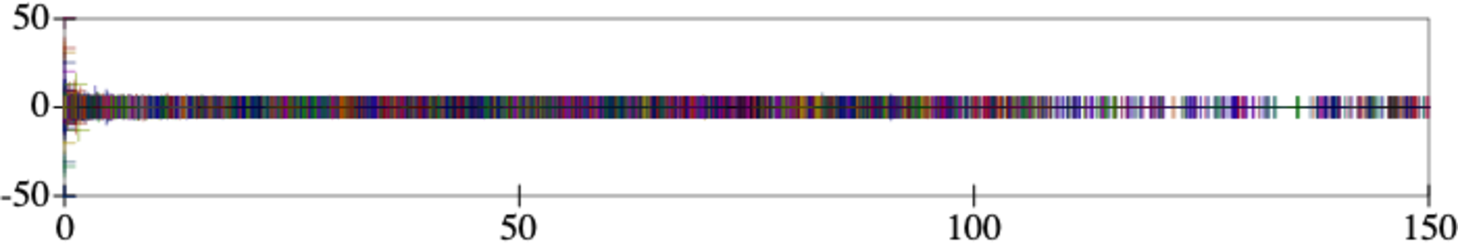
\includegraphics[width=\columnwidth]{img/error-count-nocheck-row--te-density-diff.pdf}
  \smallskip

  \mnonstrict{}
  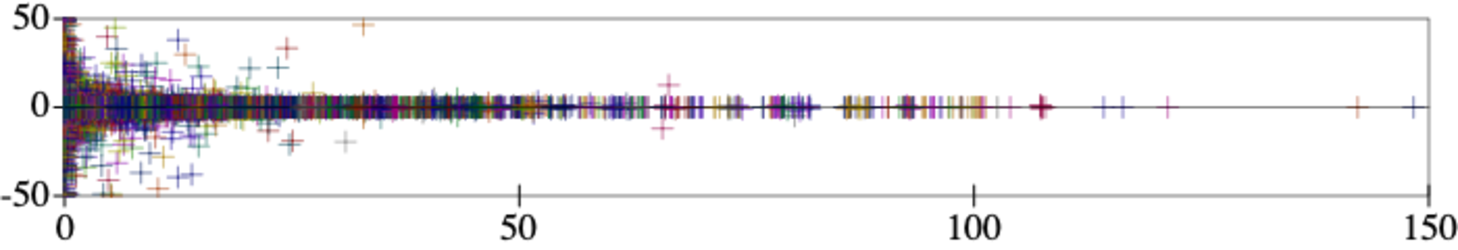
\includegraphics[width=\columnwidth]{img/error-count-nonstrict-row--te-density-diff.pdf}
  \smallskip

  \mstrict{}
  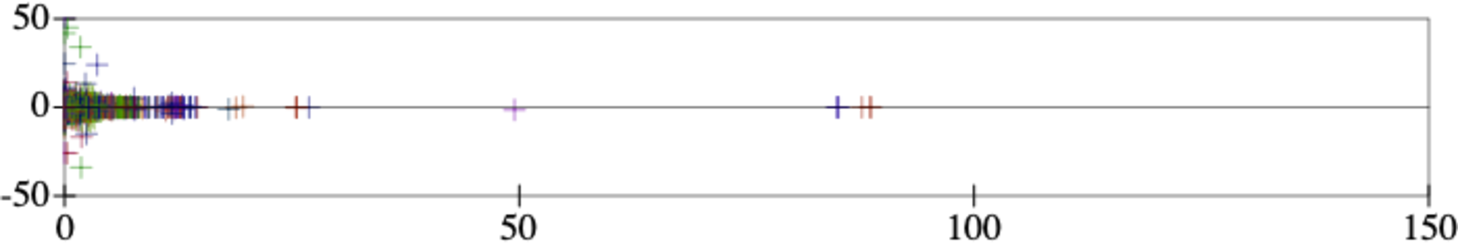
\includegraphics[width=\columnwidth]{img/error-count-strict-row--te-density-diff.pdf}
  \caption{Changes in type error density (errors in module / lines in module) over time (seconds).}
  \label{f:error-density}
\end{figure}


Moving on to type errors across the projects, and not just in the edit range,
a first interesting question is to study how the overall number of errors
changes over time.
But, the sheer number of errors can be skewed by codebase size.
To give a better basis for project-to-project comparisons, we focus
on the density of errors rather than the count, where \emph{density} is
the total number of type errors divided by the lines of code in the project.

\Cref{f:error-density} presents a zoomed-in view of type error density as it
changes over time in every session of the dataset.
The x-axis counts time in seconds from the start of the session.
The y-axis shows the change in density from the previous telemetry record
in the session to the next.
Changes can be positive or negative depending on whether the edits added
or removed errors.
The plots cut off at$\pm{}50$ density and 150 seconds.to focus on the
bulk of the data.
%% Sadly even with the zoom, it's too hard to follow one session ... the plot only gives a big-picture impression.


\paragraph{Observations}

Due to the relative adoption of type analysis, there is much more
data for the weak \mnocheck{} mode than for \mnonstrict{},
and in turn for \mnonstrict{} relative to \mstrict{}.
Still, the plots reveal interesting points:

\begin{itemize}
  \item
    All three plots are roughly balanced,
    with equal ``mass'' above and below the x-axis.
    The next section explores this point in detail.

  \item
    After the 40-second mark, changes to type error density become much
    smaller.
    Why?
    There are also fewer sessions (\mstrict{} makes that very clear).

  \item
    \mnonstrict{} has the biggest number of up/down deltas in the 10+ range.
\end{itemize}


\subsection{Do Edits Tend to Add Type Errors?}

\begin{figure}[t]\centering
  % TODO use bars instead, percent only, don't care about counts

  % TE: nocheck & 48378 & [\pct{46.83}] & 9440 & [\pct{9.14}] & 45479 & [\pct{44.03}] \\
  % TE: nonstrict & 19491 & [\pct{39.63}] & 9567 & [\pct{19.45}] & 20121 & [\pct{40.91}] \\
  % TE: strict & 733 & [\pct{39.18}] & 368 & [\pct{19.67}] & 770 & [\pct{41.15}] \\
  %
  % TE mod: nocheck & 20085 & [\pct{49.83}] & 906 & [\pct{2.25}] & 19317 & [\pct{47.92}] \\
  % TE mod: nonstrict & 13030 & [\pct{40.22}] & 5513 & [\pct{17.02}] & 13852 & [\pct{42.76}] \\
  % TE mod: strict & 419 & [\pct{39.31}] & 230 & [\pct{21.58}] & 417 & [\pct{39.12}] \\
  %
  % FS: nocheck & 270763 & [\pct{36.99}] & 238696 & [\pct{32.61}] & 222588 & [\pct{30.41}] \\
  % FS: nonstrict & 35330 & [\pct{37.28}] & 29483 & [\pct{31.11}] & 29955 & [\pct{31.61}] \\
  % FS: strict & 574 & [\pct{33.71}] & 561 & [\pct{32.94}] & 568 & [\pct{33.35}] \\
  %
  % FS mod: nocheck & 259865 & [\pct{39.09}] & 175643 & [\pct{26.42}] & 229271 & [\pct{34.49}] \\
  % FS mod: nonstrict & 33988 & [\pct{39.74}] & 20738 & [\pct{24.25}] & 30798 & [\pct{36.01}] \\
  % FS mod: strict & 488 & [\pct{36.53}] & 344 & [\pct{25.75}] & 504 & [\pct{37.72}] \\
  \begin{tabular}{l@{~}lr@{}rr@{}rr@{}r}
    & & \zerowidth{Add} & & \zerowidth{Keep} & & \zerowidth{Drop} \\\midrule
    type err. & \mnocheck{}   & 20085 & [\pct{49.83}] & 906 & [\pct{2.25}] & 19317 & [\pct{47.92}] \\
              & \mnonstrict{} & 13030 & [\pct{40.22}] & 5513 & [\pct{17.02}] & 13852 & [\pct{42.76}] \\
              & \mstrict{}    & 419 & [\pct{39.31}] & 230 & [\pct{21.58}] & 417 & [\pct{39.12}] \\
    \\
    \FS       & \mnocheck{}   & 259865 & [\pct{39.09}] & 175643 & [\pct{26.42}] & 229271 & [\pct{34.49}] \\
              & \mnonstrict{} & 33988 & [\pct{39.74}] & 20738 & [\pct{24.25}] & 30798 & [\pct{36.01}] \\
              & \mstrict{}    & 488 & [\pct{36.53}] & 344 & [\pct{25.75}] & 504 & [\pct{37.72}] \\
  \end{tabular}
  \caption{How often do edits increase, maintain, or decrease the number of errors?}
  \label{f:error-changes}
\end{figure}

The apparent visual symmetry in the density plots~(\cref{f:error-density})
suggests that edits add and remove errors with rougly equal frequency,
regardless of mode.
No matter whether a creator is using \mnocheck{}, \mnonstrict{},
or \mstrict{} mode, edits seem to balance increases and decreases in the number
of type errors.
\Cref{f:error-changes} explores this question of balance in detail.
For each of the three modes, it reports the percent of edits that increase (Add),
maintain at a nonzero level (Keep), or decrease (Drop) the number of type
errors in the project.


\paragraph{Observations}

\begin{itemize}
  \item
    The Adds and Drops are remarkably balanced: across all three modes, they are
    at most \pct{2} apart from one another.
    This confirms that changes to the number of errors are balanced.
    Creators tend to fix errors highlighted by type analysis
    even in the stricter analysis modes.

  \item
    The percentage of Keeps is somewhat high: nearly \pct{10} in \mnocheck{}
    and \pct{20} in \mnonstrict{} and \mstrict{}.
    Evidently, the mode plays a role here.
    Outside of \mnocheck{}, type errors are more likely to persist through edits.

\end{itemize}


\subsection{Two Activities: Asset Creation and Scripting}
\label{s:strict-vs-forcedstrict}

\begin{figure}[t]\centering
  %% TODO
  %% - thin bars
  %% - colors for good , bad (disagree) , neutral
  \begin{tabular}{lll}
    \mnocheck{} & \mnonstrict{} & \mstrict{} \\
    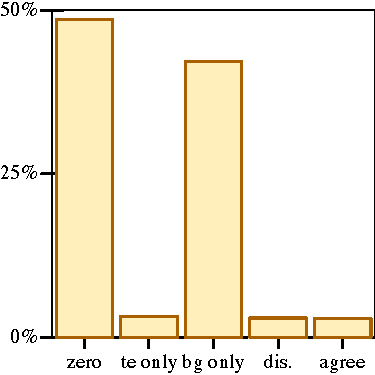
\includegraphics[width=0.3\columnwidth]{img/compass-nocheck.pdf}
    &
    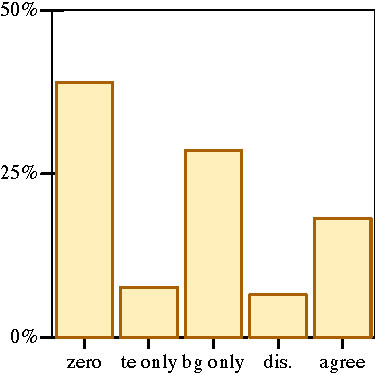
\includegraphics[width=0.3\columnwidth]{img/compass-nonstrict.pdf}
    &
    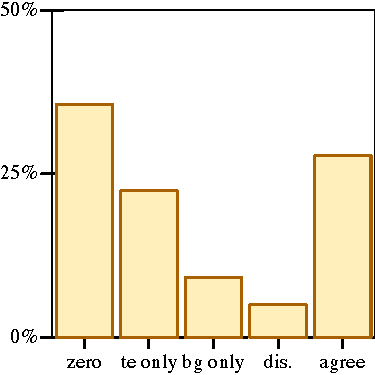
\includegraphics[width=0.3\columnwidth]{img/compass-strict.pdf}
  \end{tabular}
  \caption{Comparing the change in type errors to the change in \FS{} errors.}
  \label{f:tefs-compass}
\end{figure}

Since Roblox Studio runs each codebase through two passes of type analysis,
it is interesting to compare their results.
Of special interest is the \mstrict{} mode case, because the number of
type errors and \FS{} errors should be nearly the same.
But, there are two differences between \mstrict{} type checking
and \FS{} checking:
\begin{itemize}
  \item
    Background checks all dependencies in \mstrict{} mode, no matter
    what mode they declare.
    So, the number of \FS{} errors may be higher.
  \item
    Background checking has looser rules for the \emph{data model};
    that is, for the static assets that a program manipulates.
    So, the number of \FS{} errors may be lower.
    %% initial DM, all properties go into a table type; DM -> folder -> model -> part
    %% get dot-driven autocomplete
\end{itemize}
Our data contains a surprising number of records where \FS{}
reports fewer errors.
Data model edits are apparently a regular occurrence in Luau programs.

\Cref{f:tefs-compass} compares changes in type errors (\tekey{}) to changes in
\FS{} errors (\fskey{}) for the three analysis modes.
To a first approximation, the changes either agree with one another
or disagree.
For example, if type errors increase but \FS{} errors decrease,
we have a disagreement.
The plots futher categorize agreements and disagreements into
the following five cases:
\begin{enumerate}
  \item
    \emph{zero}: neither \tekey{} nor \fskey{} changed
  \item
    \emph{te only}: \tekey{} changed but \fskey{} remained the same
  \item 
    \emph{fs only}: \tekey{} remained the same but \fskey{} changed
  \item
    \emph{dis}: \tekey{} and \fskey{} changed in opposite directions
  \item 
    \emph{agree}: \tekey{} and \fskey{} changed in the same direction
\end{enumerate}
Both \emph{zero} and \emph{agree} are agreements.
The others are disagreements.
The plots show what percent of all telemetry records fell into these five categories.

\paragraph{Observations}

\begin{itemize}
  \item
    All three plots have a nonzero percentage of \emph{te only} items.
    In \mstrict{} mode, the percentage jumps up to nearly \pct{25}.
    Since \fskey{} is more lenient only for data model changes, these must
    be edits that affect the model in a way that raises a type error.
    Naturally, \mstrict{} mode has the largest number of such edits because
    its type checker is the most careful.

  \item
    In the first plot, for \mnocheck{},
    half the records are \emph{zero\/}s, nearly half are \emph{fs only}, and only a few
    land in the other categories.
    While the number of zeros is a bit high,
    the \emph{fs. only} spike makes sense because type checking is supposed to complain
    sparingly in \mnocheck{} mode.

  \item
    In the \mnonstrict{} plot, the number of agreements jumps up.
    This is reassuring.
    \FILL{}.

\end{itemize}

Users of \mstrict{} mode may find it frustrating that the type checker complains
about data model edits.
Though we cannot see the exact reason for the complaints, the checker errs on
the conservative side.
Thus we expect the number of useful reports is low.
This may be a barrier to adaption.


\subsection{Session Timelines}

\begin{figure}[t]\centering
  %% TODO any way to cluster timelines to avoid the "creepiness" of spying on one user?
%  \mnonstrict{}\\
%  \includegraphics[width=\columnwidth]{img/timeline-nonstrict.pdf}

  \medskip{}
  \mstrict{}\\
  \includegraphics[width=\columnwidth]{img/timeline-strict.pdf}

  \caption{Two example sessions.}
  \label{f:indy-session}
\end{figure}

Another insightful visualization that the telemetry supports is plots of individual sessions
over time.
\Cref{f:indy-session} shows the type errors, \FS{} errors, and module switches
in two \mstrict{} mode sessions.
The x-axis shows time in seconds from the start of the session.
The y-axis counts errors.
Type errors appear as orange plus marks.
Background errors appear as green x marks.
The vertical lines show module switches.

In the first plot, the error counts are low until about the 3,000s mark,
at which point an edit (not a module switch) leads to 15 errors.
These 15 errors disappear two records later.
Then, after two module switches and some edits, the number of errors spikes again.
In the second plot, the number of errors spikes in the beginning due to edits,
then remains low for the next few thousand seconds.

A general observation is that the number of type errors is always less than the number of \FS{}
errors, though the numbers are close.
This should happen in \mstrict{} mode.


\section{Answers to Research Questions}
\label{s:discussion}

With the data in hand, we can answer the research questions
from~\cref{s:introduction}.
The answers confirm several aspects of Luau's design, but
at the same time offer several directions for future improvements.
Luau clearly has a powerful typechecker that can efficiently
analyze thousands of lines of code.
But, few creators use type analysis directly and the data presents little
evidence that doing so would improve their quality of life.
We conjecture that Luau needs further tailoring to match
common idioms in Roblox scripts.
Discovering these idioms is a question for future work~(\cref{s:conclusion}).

\begin{description}
  \item[How many creators choose to use type analysis?]
    A mere \pct{10} of creators opt-in to type checking.
    Most of these use \mnonstrict{} mode, and fewer than \pct{1}
    use \mstrict{} mode.

  \item[How often do projects contain modules with different analysis modes?]
    Projects rarely combine analysis modes.
    Only 512 of \nK{340} sessions ($<\pct{1}$) switched to modules with different
    analysis modes.
    This number may be a significant underapproximation because we have data
    only on modules that the creator chose to open, but the widespread use
    of \mnocheck{} mode suggests that it is not off by much.

  \item[How often do creators turn analysis off?]
    Creators rarely disable type analysis after opting in.
    Only 233 of the \nK{340} sessions ($<\pct{1}$)
    switch to a weaker mode.
    Most of these (\pct{75}) are downgrading from \mstrict{}
    rather than \mnonstrict{} mode.
    %% FILL more insight if we match upgrades + downgrades in session?

    %% upgrade
    %% 519 total sessions
    %% 176 with up
    %% #hash((nocheck . 0) (nonstrict . 44) (strict . 132))
    %%  nocheck : 0.00\%
    %%  strict : 75.00\%
    %%  nonstrict : 25.00\%
    %%
    %% downgrade
    %% 515 total sessions
    %% 233 with down
    %% #hash((nocheck . 0) (nonstrict . 64) (strict . 169))
    %%  nocheck : 0.00\%
    %%  strict : 72.53\%
    %%  nonstrict : 27.47\%


  \item[For modules that use type analysis:]\leavevmode
    \begin{description}
      \item[- Which errors arise?]
        Syntax errors are extremely common~(over \pct{50},~\cref{t:type-error-count}), 
        followed by type mismatches~(\pct{20} in \mstrict{}),
        arity errors~(\pct{2}),
        and failure to unpack on optional value~(\pct{2}).
        There are several uncommon errors, such as misusing a table operation,
        and a few that never arise: internal and too-complex errors,
        duplicating or swapping a generic parameter, use of a deprecated API,
        and unsafe dynamic property lookup on a class.

      \item[- How do creators respond? Which errors persist through edits?]
        Creators typically fix analysis errors.
        With few exceptions, increases and decreases in the number of errors
        balance out~(\cref{f:error-changes,t:type-error-survival,}).
        Even in \mnocheck{}, most edits that overlap with syntax errors
        remove at least one error~(\pct{67}) rather than increase or maintain
        the total.
        The errors that most-often survive edits are due to
        inference at a binary operation,
        sending \code{self} to a function that does not expect it,
        and failure to unpack an optional value.
        But the first two seldom arise, and the third is something creators
        might reasonably ignore while prototyping.

%% Keep percents
%% '((CannotInferBinaryOperation "0.50")
%%   (OptionalValueAccess "0.44")
%%   (FunctionDoesNotTakeSelf "0.40")
%%   (CannotExtendTable "0.35")
%%   (UnknownPropButGotLikeProp "0.28")
%%   (UnknownProperty "0.26")
%%   (MissingProperties "0.25")
%%   (FunctionExitsWithoutReturn "0.21")
%%   (ModuleHasCyclicDependency "0.20")
%%   (UnknownRequire "0.18")
%%   (TypeMismatch "0.18")
%%   (UnknownSymbol "0.15")
%%   (NotATable "0.12")
%%   (GenericError "0.11")
%%   (CannotCallNonFunction "0.10")
%%   (CountMismatch "0.09")
%%   (GenericExtraInformation "0.07")
%%   (IllegalRequire "0.06")
%%   (SyntaxError "0.01")

    \end{description}

  \item[What impact does type analysis have on the number of \FS{} errors?]
    Opting in to type analysis has little impact on \FS{} errors.
    The percent of \FS{} errors in \mnocheck{} code matches the percent of
    creators using \mnocheck{} mode~(\cref{f:error-by-mode}); whereas,
    if type analysis helped reduce \FS{} errors, \mnocheck{} would own a
    higher percentage of the errors.
    Furthermore, there is no apparent relation between \FS{} errors and edits,
    regardless of analysis mode~(\cref{f:error-changes}).
    A randomly-chosen edit has a 1/3 chance of increasing, decreasing, or
    maintaining the number of \FS{} errors.

\end{description}


\paragraph{Threats to Validity}
\label{s:threats}

While this study has high ecological validity due to its focus on
working creators, there are several threats to keep in mind.
Some threats stem from our method of collecting data; others
come from the limited scope of the data.

First of all, sampling is necessarily incomplete.
Though the data includes many thousands of sessions, it
may have missed a few critical sessions where a creator
adopted \mstrict{} mode, encountered \code{CodeTooComplex} errors,
and gave up.
Furthemore, our method of sampling by keystroke and by module switch
skews the data toward creators who, for whatever reason, do more
of these actions.
We have no access to other events (e.g., run locally, publish) due to privacy
concerns; future studies may wish to avoid this limitation by actively
recruiting subjects.

Second, the edit ranges are a coarse approximation of actual edits.
They begin at the lowest edited line of code and end at the highest
edited line, even if nothing between those lines changed.

Third, the total counts of type errors include a large number of syntax errors,
which have little to do with the Luau type system and are presumably easy for
creators to fix.
It would be better for the analysis to ignore these errors.
Indeed, our comparison between \FS{} errors in \mnocheck{} vs.
\mstrict{} mode~(\cref{f:error-changes}) might tell a very different story
without all the noise that syntax errors introduce.

Fourth, type analysis reports several errors at once and we have no idea which
errors, if any, creators intended to fix with their edits.
Although it appears that creators choose to fix errors with their edits,
the fixes may be a side effect of other plans.

% Telemetry cannot replace user studies, as there is no way to measure
% creator sentiment, but provide complementary data at scale.
% No idea about intent is a big problem, we don't know which error the creator wanted to fix.

Lastly, we have two remarks about external validity.
First, our information on type errors is limited to error names.
If another language has an error that is roughly similar to the
\code{CannotCallNonFunction} error but with slightly different
semantics, then the relative frequency of that error could be different
than what we observed.
Second, we know nothing about the creators in our study except that they
were selected at random from a large and diverse group.
A dataset based on a targeted subset of users might show entirely different
characteristics.


\section{Related Work}
\label{s:related}

\begin{table}[t]\centering
  \caption{Comparison of telemetry designs. Two orthogonal concerns are \emph{when} to collect data and \emph{whether} to add noise to enhance privacy.}
  \label{t:telemetry-design}

  \begin{tabular}{l@{~~}c@{~~}c@{~~}c@{~~}c@{~~}c}
    ~             & Event Counts & Timestamps & Error Msgs. & Source Code \\\midrule
    Roblox Studio & \chkYes      & \chkYes    & \chkNo        & \chkNo    \\
    Transparent   & \chkYes      & \chkNo     & \chkNo        & \chkNo    \\
    Classic       & \chkYes      & \chkYes    & \chkYes       & \chkYes   \\
  \end{tabular}
\end{table}

% kindle track every tap (page turn etc),
% enables whispersync feature,
% drove design of navigation tools,
% opt-out possible~\cite{kindle-telemetry}

Type error telemetry in Roblox Studio has two distinguishing characteristics:
it includes no personal information (PII), and it sends data on
randomly-selected runs of the type checker rather than specific events of interest.
To the best of our knowledge, this design occupies a unique position relative to prior
work~(\cref{t:telemetry-design}).

In other professional-grade IDEs, such as VSCode~\cite{vscode-telemetry}
and \code{.NET}~\cite{dotnet-telemetry}, telemetry may include all sorts of
data: error reports, source code fragments, timestamps, and filepaths.
Users may be able to opt out of some telemetry, but the details depend on the
license agreement.
Furthermore, at least in VSCode, IDE extensions can report their own telemetry.
While this data can be invaluable for discovering bugs in production, it
must be handled with extreme care.

The Blackbox project similarly collects telemetry in broad strokes.
Every Java program submitted for compilation goes into the Blackbox database (minus
any comments above the main class) along with the compiler's response~\cite{bkmu-sigcse-2014}.
%% Though somewhat intrusive,
The millions of programs in the Blackbox dataset
have enabled dozens of contributions to the area of CS
education~\cite{bask-icer-2018}, ranging from categorization of novice
errors~\cite{mk-fie-2014,m-masters-2016} to analyses of error frequency and
time-to-fix~\cite{ab-sigcse-2015}.
Related prior work used the GRUMPS telemetry system to collect 4.7 million
keystroke-level actions from learners programming in
Ada~\cite{tm-iticse-2004,tkdmceg-ascilite-2003}.
This data is not available.

At the opposite end of the privacy spectrum, Go's design for \emph{transparent
telemetry} reports only counter values~\cite{transparent-telemetry}.
Unlike Roblox Studio, transparent telemetry includes no timestamps and no 
session ids.
The data is useful for learning about the frequency of specific events and the
distribution of events across clients (e.g., how many \code{CodeTooComplex}
errors arise? what is the average number of type errors?).
However, the lack of timestamps and ids means that it cannot track edits
over time (a feature that is quite useful to us, for example, in~\cref{f:error-density}).
% In~\cref{f:error-density}, for example, we see that increases to the number
% of type errors are quickly followed by decreases.
% Without timestamps, we would be unable to rule out the possibility that users
% build up a mountain of type errors and then slowly reduce them to zero.


\paragraph{Telemetry Enhancements: What and How to Sample}

One way to futher strengthen the privacy of any telemetry design, including
transparent telemetry, is to systematically add noise to the data using
techniques from differential
privacy~\cite{zhlbr-cc-2020,epk-ccs-2014,wblj-usenix-2017}.
Recent work that is especially relevant to the session-based data collected
by Roblox Studio shows how to add noise to traces~\cite{zhlbr-cc-2020},
how to account for known relationships between events~\cite{zhlbr-oopsla-2020},
and how to choose the noise amount on the client side~\cite{hlzbr-ecoop-2021}.
Applying differential privacy is subtle, however.
While we can likely fuzz the total number of type errors, if we were to
fuzz the number of \code{CodeTooComplex} errors, it might drastically
affect our conclusions.

Cooperative bug isolation is a method for designing
telemetry systems~\cite{liblit-thesis}.
The focus is not on privacy, but rather on how to collect a small amount of
data from each user and perform statistically-sound analyses.
Each feature of interest \emph{within} a user's codebase has a uniform-random
probability of contributing telemetry.
The system-builder can analyze this telemetry with predicates to identify
notable events and logistic regression to narrow down nondeterministic bugs.
There is a high burden on designers to decide what to capture,
but a careful design can minimize the data from each individual user.
%% more in diss: how to deal with native compilers, threads, dynamic loading
%% ... privacy is future work, can maybe avoid private data with a type system

Two further refinements, which reduce the burden on experts to
select points of interest, are adaptive bug isolation~\cite{nl-icse-2010}
and blame-proportional logging~\cite{lnsmc-usenix-2018}.
Adaptive bug isolation starts with a set of predicates, studies which are
most correlated with failures, and experiments with adding telemetry to nearby
predicates; this technique can reduce the overhead of telemetry by two orders
of magnitude relative to naive binary instrumentation.
Blame-proportional logging starts with lightweight telemetry to recognize
defects, assigns ranks to methods estimating their likelihood as root causes,
and uses the ranks and future observations to narrow down the cause.
Deep transfer learning is another promising way to hone in on events of
interest~\cite{zfstt-ieeesensors-2022}.

%% \cite{fnm-sigmod-2020}
%% adaptive interventional debugging
%% failure -> correlated predicates -> temporal properties to overapprox relationships -> fault injection to discover true relationships

%% RAMSS workshop (remote measurement), sounds related but i haven't found proceedings
%% \cite{op-ramss-2003,op-ramss-2004}


\paragraph{User Studies, Errors, and Type Errors}

Our approach to data analysis is inspired by Marceau
et~al.~\cite{mfk-onward-2011,mfk-sigcse-2011}, who used keystroke-level data
collected over 6 weeks to analyze students' responses to runtime errors
in DrRacket~\cite{fcffksf-jfp-2002}.
Similarly, Macedo et~al.~\cite{mcpcsprs-abz-2020,mcpcsprs-scp-2021} capture
edit sessions from the online Alloy4Fun editor and present several automated
analyses.
A major challenge in our setting, however, is that edit sequences are
incomplete---there may be minutes-long gaps between two telemetry records.
Several more-recent works have studied edit sequences
to draw conclusions about errors and intent, e.g.,~\cite{wk-koli-2020,lgk-pj-2022,rsgl-cpp-2020}.

The BitFit project collects data about beginning students interactions with a
Java IDE~\cite{ekc-wccce-2016,anna-russo-kennedy-ms-2006}; however, unlike Blackbox, it does
not collect source code.
BitFit data consists of a timestamp, a session id, and counter values showing
the number of attempts at a question, the number of hints requested, the number
of compiles and runs, and the number of submission attempts.
On one hand, this data is more informative than Roblox Studio's because it
targets specific events rather than random keystrokes.
On the other hand, there are no details about errors to show what students
struggled with.
Other logging-based studies of Java programs use the full error message to
draw conclusions~\cite{bgimgm-cse-2016,dlc-iticse-2014}.
Roblox Studio cannot follow this approach because strings in errors may leak
personal information.

Much work on the benefits of static types focuses on a small number
of case studies~\cite{w-popl-1986,hw-scp-2004,td-tosem-2001},
inverviews~\cite{cdhhjklwya-hatra-2020,gstf-hatra-2021,cams-oopsla-2020},
or static corpuses~\cite{rppd-fse-2014,bhmvv-toplas-2019,bmvv-arxiv-2019}
(for literature reviews, see~\cite{empirical-types,heeren-thesis}).
Controlled experiments, for example comparing statically-typed Java and dynamically-typed
Groovy~\cite{khrts-icpc-2012}, are a notable exception.
Lerner et~al.~\cite{lfgc-pldi-2007} apply type error repair tool on over two thousand
of programs written during five homework exercises.
Seidel et~al.~\cite{sscwj-oopsla-2017,sjw-jfp-2018} use five thousand programs
to train data-driven methods for localizing errors.
These large studies with several thousands of programs are
nevertheless on a much smaller scale than Roblox Studio.

%\paragraph{TBD}
%
%ahmadzadeh elliman higgins iticse 2005
%
%buffardi etal 2014 adaptive and social mechanisms
%
%bddf-icse-2016
% sh edwards and jason snyder icer 2009 comparing effective and ineffective grading platform
%
%murphy etal sigcse 2009 Retina: helping students
%
%Choppella Haynes IU TR 426

% ESP workshop on empirical studies of programming
% https://dl.acm.org/doi/proceedings/10.1145/266399
% nothing sounds big ... empirical yes, large no
% https://link.springer.com/content/pdf/10.1023/a:1008040416962.pdf

% \cite{}
% heeren
% constraint-based type inference;
% general te criteria:
% - target audience (novice / expert)
% - output format (text / viz)
% - interactivity (yes / no)
% - heuristics (yes / no)
% - primary-or-external (most type errors are easy, some could really use dedicated help)

% \cite{t-hatra-2021}
% plan for a large user-centered study of proof assistants,
% events: up, down, to cursor, interrupt, reset.
% ... not very deep, look at edit sequences, replay for errors


\section{Lessons Learned and Reflections}
\label{s:conclusion}

This paper presents the first large-scale analysis of developers' interactions with
an industrial strength typechecker.
With over 1.5 million telemetry records from over 300,000 sessions
that took place during a three-month timespan, the data has plenty to say about
type errors and their overlap with program edits.
At the same time, the data is carefully restricted to avoid leaking personal
and proprietary information: we know the number and kind of type errors
that occurred, but nothing about the line(s) of code that the typechecker
complained about.

On the object level, the analysis offers several lessons for the Luau
developers and other maintainers of gradually-typed languages:
\begin{itemize}
  \item
    Nearly all creators (\pct{90}) use the default ``no check''
    typechecking mode~(\cref{f:dataset-overview}).
    Since the next typing mode (\mnonstrict{}) requires no annotations and is
    very conservative about the errors it reports, we conjecture that
    developers would have no objections to using it and are simply unaware that
    other modes exist.
%  \item
%    \pct{50} of all errors are in current module, so probably errors appear locally (not in a distant module);
%    \pct{5} of (current? old??) type errors overlap with edit range, so they don't stick around.
  \item
    Creators tend to fix errors immediately rather than dealing with them in a batch
    or ignoring the errors altogether~(\cref{f:error-density,f:error-changes}).
    % Changes to the number of errors balance one another~(\cref{f:error-density});
    % edits are equally likely to add or remove errors~(\cref{f:error-changes}).
  \item
    All Luau scripts interact with data assets, but no typechecking mode
    has a precise view of the data.
    Improving precision is an important direction for future work.
    Until then, \mstrict{} mode clearly needs to relax its data model
    analysis because it raises even more errors than \FS{} checking~(\cref{f:tefs-compass}).
\end{itemize}


On the meta level, the main takeaway is that the lightweight, counter-based telemetry
in Roblox Studio supports a variety of useful analyses:
\begin{itemize}
  \item
    Counting specific type errors helps to identify trends and to confirm that
    undesirable events rarely happen (e.g.,\code{UnificationTooComplex}).
  \item
    Testing the relationship between two counts can yield insights.
    The gap between \mstrict{} and \FS{} errors In~\cref{f:tefs-compass}
    revealed an issue with \mstrict{} checking.
  \item
    Reporting the overlap between type errors and the current (approximate) edit
    range lets us assess the outcome of edits without revealing source code.
    It was especially useful to have overlaps for two sets of type errors: old and current.
  \item
    Timestamps give useful, low-level insights about the frequency of keystrokes,
    the length of sessions, and actions over time~(\cref{f:indy-session}).
    The event ordering that timestamps provide was invaluable; e.g., for learning
    that error deltas bounce up and down rather than rising shaply, then falling~(\cref{f:error-density}).
\end{itemize}

One aspect of the telemetry that we would change for next time is to provide
more metadata.
Luau recently adopted semantic subtyping to reduce false-positive type
errors~\cite{CF05:GentleIntroduction,Jef22:SemanticSubtyping}, but the current
telemetry has no way to tell if this
internal extension is enabled or not.
Three other aspects are worth rethinking.
First, it would be useful to have fine-grained counts for \FS{} analysis
errors and to know the specific reason behind errors such as \code{TypeMismatch}.
But, this additional data could double the size of telemetry records.
Second, although tracking edit ranges was useful, it made the telemetry system
much more difficult to build and maintain.
Tracking old and current errors at the module level would be far easier,
though there is a risk that it is too coarse.
Third, the massive number of syntax errors begs the question of how to skip
them.
Shifting focus from arbitrary keystrokes to selected ones, such as closing
parentheses or whitespaces, might increase the likelihood of well-formed
code without losing the ``middle of things'' nature of the data.
Another option is to ignore records that have a syntax error in the edit range.

In future work, it would be interesting to build statistical models of
the ``average'' programmer using each typing mode and compare their error
rates.
While one could start modeling with the \mnocheck{} and \mnonstrict{}
data, but there are too few \mstrict{} records at the moment due to our uniform
sampling rate.
The errors that we do see in \mstrict{} mode call for an in-depth analysis via
talk-aloud interviews to discover why type mismatches occur and how how Luau
can better accommodate untyped idioms.


%% PS
%% - downloading from Kibana was a HUGE pain and source of errors. Awful!
%% - worth finding ways to reduce / ignore syntax errors?


%% -----------------------------------------------------------------------------
\acks

Thanks to Benjamin Chung for several helpful discussions about data analysis
and effective plotting.
Greenman was supported by
NSF grant \href{https://nsf.gov/awardsearch/showAward?AWD_ID=2030859&HistoricalAwards=false}{2030859}
to the CRA for the \href{https://cifellows2020.org}{CIFellows} project.

%\newpage
%
%\appendix
%
%\section{Data Details}
%
%Tips for interpreting the data:
%
%\begin{itemize}
%  \item
%    Edit ranges are non-negative because we
%    implemented the interval arithmetic for them using unsigned integers.
%    To filter out negative edit ranges, we removed all ranges
%    greater than 4 billion.
%
%  \item
%  \item
%  \item
%\end{itemize}
%
%\newpage

\bibliography{bib}

\end{document}
